%%%%%%%%%%%%%%%%%%%%%%%%%%%%%%%%%%%%%%
\chapter{REDIRECTION OF SOUND BY A PERIODIC CHAIN OF PERFORATED METALLIC CYLINDRICAL SHELLS}
%%%%%%%%%%%%%%%%%%%%%%%%%%%%%%%%%%%%%%

%%%%%%%%%%%%%%%%%%%%%%%%%%%%%%%%%%%%%%%%%%%%%%%%%%%%%%%%%%%%%%%%%%%%
\section{Introduction}

This chapter provides insights into the~phenomena of sound manipulation that are achievable with the~periodic chain of highly symmetric scatterers.

It is known that in the~case of electromagnetic waves, such chains composed of cylinders or spheres may serve as waveguides \cite{quinten,brongersma,maier}. They can also efficiently transverse electromagnetic energy provided the~scatterers are close enough so that they couple via the~plasmonic near-field.
However, in such structures, especially in linear chains, the~dissipation of energy may be quite large as there are not only the~Joule losses, but also the~radiative \cite{ford,papanikolaou,markel,malyshev,vergeles} and collisionless nonradiative \cite{jalabert} losses (Landau damping).

In acoustics, one cannot achieve very strong coupling between two neighboring scatterers as it would require the~existence of some analog of the~gap plasmon resonance.
Still, the~fact that it is much easier to manipulate the~density, elasticity, and viscosity of the~media than their dielectric permittivity, allows predicting and observing transport properties specific for acoustic waves.

\subsection{Phenomena in Periodic Arrangements of Scatterers}

Earlier studies of the~periodic chains where the~scatterers had internal structure (basically, mass-in-mass units) demonstrated that such scatterers exhibit negative mass density and the~mechanical energy can be guided along the~chain \cite{huang1}.
In the~case of elastic mass-in-mass units having lateral resonances, the~chain was predicted to exhibit the~metamaterial behavior, with both the~effective mass and the~elastic modulus being negative \cite{huang2}.
Also, the~negative effective index of refraction for sound waves can be achieved, as was shown in \cite{kaina} for the~structure containing two acoustic Helmholtz resonators (soda cans) per unit cell of the~chain.
This becomes possible if the~dispersion of the~chain is engineered to have its passing band within a~hybridization gap.
Other examples \cite{haberman,cummer} demonstrate as well that once the~acoustic interactions between scatterers is sufficiently strong, the~system amasses a~variety of metamaterial properties.

Now, the~scatterers do not necessarily have to be built to feature strong coupling.
In fact, periodic structures with artificially {\it weak} scatterers may be of great interest for researchers, since the~interference between the~scattered waves from a~single unit and the~collective wave motion resulting from periodicity allows observation of some very delicate effects \cite{martin}.
As an~example, \cite{norris1} predicts a~Poisson-like effect in the~scattering of sound by a~periodic composition of cylindrical shells, where the~acoustic energy experiences a~$90^{\circ}$-redirection of its direction of propagation.
Responsible for such effect is the~resonant excitation of an~antisymmetric mode with polarization perpendicular to the~direction of incoming sound.
In an~elastic solid, a~behavior similar to the~Poisson effect is exhibited by a~cylindrical surface displacing periodically at the~resonance, elongating while being squeezed and vice versa.
In order to excite the~antisymmetric mode, one needs to alter the~sound-matter interaction by switching off its strongest monopole and dipole contributions, which can be achieved by matching the~density and elastic modulus of the~solid shell to those of the~background fluid \cite{norris2,norris3}.
The~interactions are thus occurring via the~nonisotropic quadrupole term, which leads to the~excitation of the~normally deaf antisymmetric collective mode and, ultimately, to the~generation of sound waves in the~direction perpendicular to the~incident wave \cite{norris1}.
It is worth mentioning that the~weakness of scattering is not itself responsible for the~Poisson-like effect, yet it poses as a~necessary condition for its observation.

\subsection{Redirecting Acoustic Antenna from Weak Scatterers}

A~similar effect of $90^{\circ}$-redirection of sound by a~linear chain of perforated metallic cylindrical shells was predicted in \cite{garcia1}, however, the~physical reason behind it is quite different.
Any perforated shell behaves as a~weak scatterer when the~thickness of the~viscous layer in the~surrounding fluid is much smaller than the~size of perforations. %$\delta = \sqrt{\eta_0/\rho_0 \,\omega}$, where $\eta_0$ is the~dynamic viscosity of the~fluid, $\rho_0$ is the~fluid density, and $\omega$ is the~frequency of sound, is much smaller than the~size of perforations.
This makes the~considered chain practically transparent for the~normally incident sound as the~weakly scattering shells have no internal resonances (at least, in the~kHz frequency range) \cite{garcia1}.
Nevertheless, for the~frequencies associated with the~Wood's anomaly, i.e., when the~wavelength of sound closely matches the~period of the~chain, the~transmission becomes anomalously low.
In this chapter, I will examine the~microscopic mechanism behind such low transmission and show that the~primary cause of the~effect is the~resonant interaction of the~incoming sound with the~symmetric leaky eigenmodes of the~chain.
Specifically, I will consider scattering of incoming plane waves by a~linear chain of perforated cylindrical shells (with the~parameters similar to those in \cite{garcia1}) with either finite or infinite number of scatterers in both ideal and viscous fluids.

\subsection{Properties of the~Redirecting Antenna}

There are, however, several properties of the~system that can be deduced immediately.
First of all, the~dispersion equation, which is yet to be derived for the~eigenmodes of the~chain, will undoubtedly produce the~band structure similar to that in the~empty-lattice model, as the~scattering on every unit is weak.
The~dispersion will then be practically linear, and the~eigenmodes will propagate with the~speed equal to the~speed of sound in the~background fluid, except for the~vicinity of the~points of degeneracy (the~$\Gamma$-point and the~edges of the~Brillouin zone) where the~level repulsion yields a~doublet of levels.
The~two eigenfunctions describing to the~components of the~doublet are symmetric and antisymmetric functions of coordinates, respectively.
It is known that only the~symmetric mode can be excited at normal incidence, while the~antisymmetric one becomes a~deaf mode \cite{jose,ward}.
When the~frequency of the~external wave matches the~eigenfrequency of the~symmetric mode, the~transmission of sound is strongly suppressed as the~eigenmode is resonantly excited.

In general, only when the~spectrum of eigenfrequencies is complex, the~external plane wave can excite the~eigenmodes.
Such modes with complex eigenfrequencies are the~so-called leaky modes which carry the~acoustic energy away into the~background fluid.
If the~imaginary part of the~frequency is small, the~acoustic energy is mainly transmitted along the~chain, meaning that the~the~part of the~initial energy flux is redirected by $90^{\circ}$.
The~effects of redirection of sound were studied for periodic systems of scatterers \cite{garcia1,norris1,deraa1}, and similar effect exists for a~narrow fluid channel between two solid elastic plates, as was discussed in the~previous chapter.

One can also resonantly excite both symmetric and antisymmetric modes by an~obliquely incident wave.
No matter how small the~angle of incidence, the~nonzero component of the~wave vector along the~chain ensures that the~incoming front does not have any symmetry and thus there is no restriction as to which mode can be excited and which cannot.
In addition, addressing the~properties of the dispersion law for the~eigenmodes is crucial.
Namely, the~dispersion of each level in the~empty-lattice model alternates between normal and anomalous, the~property which is preserved in the~1D system with weak periodic scattering potential.
Near the~$\Gamma$-point, the~upper (high-frequency) level of the~doublet exhibits normal dispersion, whereas the~dispersion of the~lower (low-frequency) level is anomalous.
The~phase and group velocities in the~case of normal dispersion are parallel, and in the~case of anomalous dispersion --- anti-parallel.
This dictates an~essentially different behavior for the~scattered waves for the~two frequencies of the~doublet.

Since the~excitation of the~eigenmode in the~chain occurs when its Bloch vector $\mathbf{q}$ matches the~parallel component $\bf k_{||}$ of the~wave vector in the~incoming wave, and since the~group velocity indicates the~direction of propagation of acoustic energy, the~eigenmode with normal dispersion will carry energy in the~direction of $\bf k_{||}$ along the~chain.
The~mode with anomalous dispersion, on the~contrary, redirects energy to run against $\bf k_{||}$ along the~chain.
For the~small angle of incidence, the~two levels of the~doublet are close to each other, thus enabling the~chain of perforated shells to serve as a~splitting antenna.
An~incoming signal consisting of two harmonics matching the~doublet frequencies will have its higher- and lower-frequency components redirected by such antenna by almost $90^{\circ}$ with respect to their original direction and in the~opposite directions to each other.
The~anticipated phenomena are robust with respect to the~viscosity of the~fluid, with the~only differences being quantitative, not qualitative, provided the~viscosity is not too large.

%\textcolor{red}{change below}

%For this purpose, we develop a~theory of scattering of external plane waves by a~linear chain of perforated cylindrical shells with finite and infinite numbers of scatterers in viscous \textcolor{red}{and ideal (inviscid)} fluid. A~method of expansion over cylindrical waves applied here leads to an~infinite set of linear equations for partial transmission and scattering amplitudes. Also, a~transcendental equation for the~dispersion law of the~eigenmodes is derived and numerically solved for the~few lowest bands. Because of weak scattering, the~band structure is close to that obtained in the~empty-lattice model. Away from points of degeneracy, the~dispersion is practically linear with speed equal to the~speed of sound in the~background fluid. However, at the~$\Gamma$-point and at the~edges of the~Brillouin zone the~doublets of levels are formed due to level repulsion. The~eigenfunctions corresponding to the~components of the~doublet are either symmetric or antisymmetric functions of coordinates. Since at normal incidence only the~symmetric mode can be excited, the~antisymmetric mode turns out to be a~deaf mode \cite{jose,ward}. At normal incidence, a~sharp minimum in the~transmission spectrum appears when the~frequency of the~external wave coincides with the~frequency of the~symmetric component, which turns out to be the~lower level of the~doublet.

%Excitation of the~eigenmodes by an~external plane wave is possible since the~spectrum of eigenfrequencies is complex, i.e., all the~eigenmodes of a~linear chain are leaky modes radiating acoustic energy into the~background fluid. An~excited eigenmode transmits energy along the~chain, i.e., the~initial flux of energy is partially redirected by $90^{\circ}$. The~effect of redirection of acoustic energy was recently predicted not only for periodic systems of scatterers \cite{garcia1,norris1,deraa1} but also for a~narrow fluid channel in a~solid elastic plate \cite{channel1,channel2}.

%Resonant interaction of the~external wave with both eigenmodes -- symmetric and antisymmetric -- can be realized at oblique incidence. Even at small angles of incidence, the~symmetry of the~incoming front is broken by a~nonzero component of the~wave vector $\bf k_{||}$ along the~chain which allows excitation of the~antisymmetric eigenmode. In 1D system with weak periodic potential the~high-frequency component of a~doublet near the~$\Gamma$-point exhibits normal dispersion. Unlike this, the~dispersion is anomalous for the~low-frequency component (phase and group velocities are anti-parallel). Due to this difference the~scattering patterns for two close frequencies in a~doublet look very different. Excitation of any eigenmode in the~chain requires matching of the~Bloch vector of this eigenmode $\bf q$ and the~parallel component $\bf k_{||}$ of the~wave vector in the~incoming wave. The~direction of propagation of acoustic energy is given by the~vector of group velocity. For the~symmetric mode possessing anomalous dispersion the~redirected energy propagates against $\bf k_{||}$, and for the~antisymmetric mode with normal dispersion the~energy runs in the~direction of $\bf k_{||}$. Since at small angles of incidence the~matching condition $\bf k_{||}=q$ is satisfied for close frequencies, a~chain of perforated shells may serve as a~splitting antenna that redirects the~higher-frequency harmonic of incoming signals along the~direction of $\bf k_{||}$ and the~lower-frequency harmonic in the~opposite direction. Our calculations show that anomalous scattering, redirection, and splitting of sound are robust with respect to viscosity. In particular, the~viscosity of air does not undermine the~pattern of anomalous scattering.



%%%%%%%%%%%%%%%%%%%%%%%%%%%%%%%%%%%%%%%%%%%%%%%%%%%%%%%%%%%%%%%%%%%%
\section{Single Scatterer Characterization}

\begin{figure}
\begin{center}
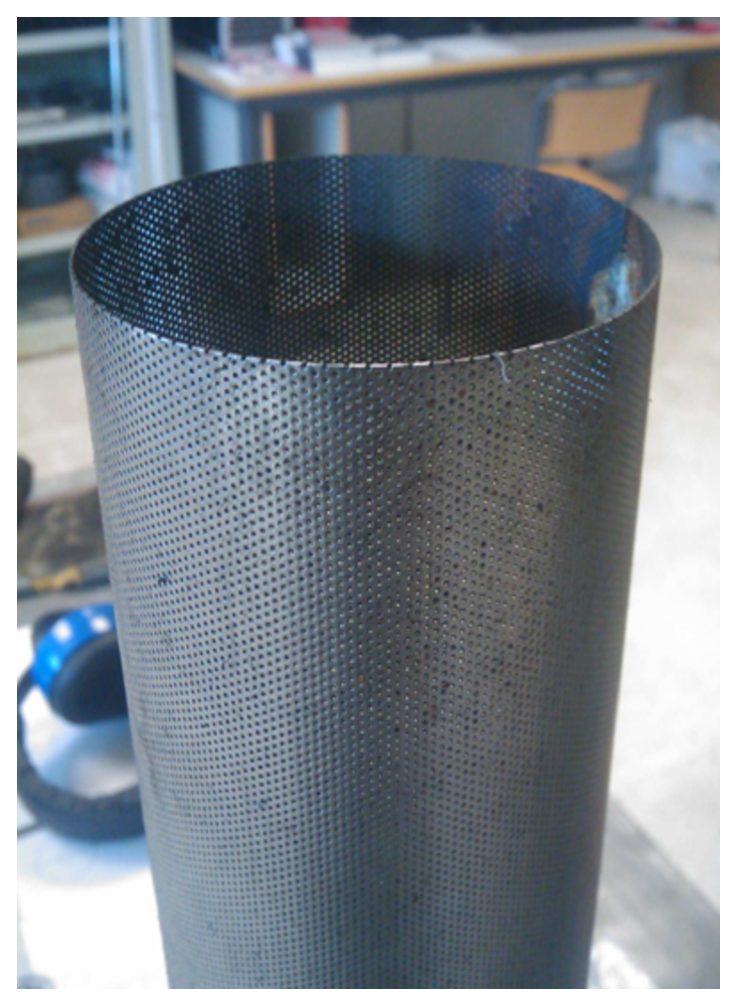
\includegraphics[width = 0.7\linewidth]{singleshell.eps}
\caption{The~perforated metallic cylindrical shell fabricated and used in the~experiments in \cite{garcia1, garcia2, garcia11}.}
\label{fig:singleshellChain}
\end{center}
\end{figure}

Each cylindrical shell is produced by rolling a~perforated metal plate into a~cylindrical shape (see \cref{fig:singleshellChain}).
In this chapter, I will be using the~same material and geometry parameters that were adopted for the~experimental and numerical studies in \cite{garcia1, garcia11}, namely:
\begin{equation*}
\hspace{-5cm}
\begin{array}{lll}
\bullet &\text{outer radius of the~shell} &a=4.00 \text{ cm},\\
\bullet &\text{inner radius of the~shell} &b=3.95 \text{ cm},\\
\bullet &\text{thickness of the~shell } (h=a-b) &h=0.05 \text{ cm},\\
\bullet &\text{radius of the~circular perforation} &r = 0.25 \text{ mm},\\
\bullet &\text{filling fraction of the~perforations} &\sigma = 0.145.\\
\end{array}
\end{equation*}


The~metal from which the~shells were made of was aluminum, and the~parameters of the~air environment are as follows:
\begin{equation*}
\hspace{-6.5cm}
\begin{array}{lll}
\bullet &\text{density of air} &\rho_0=1.25 \text{ kg/m}^3,\\
\bullet &\text{speed of sound in air} &c_0=343 \text{ m/s},\\
\bullet &\text{viscosity of air (dynamic)} &\eta_0 = 17.8\,\mu\text{Pa}\cdot\text{s}.\\
\end{array}
\end{equation*}

The~interaction of the~perforated shell with the~sound, specifically, the~boundary conditions at the~metal-air interfaces, will be described by the~effective impedance $Z_p$ of the~shell.


\section{Impedance of the~Perforated Scatterer}

The~notion of effective impedance was introduced in the~works \cite{maa,maa2} for flat thin perforated plates, and it differs essentially from the~notion of the~acoustic impedance of the~medium $Z=\rho c$.
For a~plate of thickness $h$ coinciding with the~$xOy$ plane, the~effective impedance was defined as
\begin{equation}
\label{eq:impedanceChain}
Z_p~=~\frac{\left.p\right|_{z=-\frac{h}{2}}-\left.p\right|_{z=+\frac{h}{2}}}{\bar{v}_z},
\end{equation}
where the~pressures in the~numerator are evaluated on either side of the~plate, and the~denominator expresses the~$z$-component of the~average velocity of the~fluid inside the~perforation.

This idea of the~effective impedance comes with additional assumptions.
First of all, it relies on the~high contrast between the~material of the~plate and the~environment.
This condition is satisfied when experimenting with metal plates in air, and therefore one may assume the~metal regions to be ideally rigid.
Then, the~transmission of sound through the~perforated plate occurs mostly through the~perforations.
The~plate is assumed to be perforated uniformly with a~quite high perforation constant, so that a~single boundary condition would apply for the~entire plate regardless of where the~openings are actually located.
This boundary condition takes the~form of
\begin{equation}
\label{eq:bcChain}
\left.v_z\right|_{z=-\frac{h}{2}}~=~\left.v_z\right|_{z=+\frac{h}{2}}~=~\frac{\left.p\right|_{z=-\frac{h}{2}}-\left.p\right|_{z=+\frac{h}{2}}}{Z_p},
\end{equation}
where due to the~small thickness of the~plate the~velocities on either side of the~plate are approximately equal.
Also, the~wavelength of sound that penetrates through the~plate must be much larger than the~perforation size.

The~expression for $Z_p$ through the~material parameters and the~perforation geometry is typically represented as a~sum of internal and external terms which capture different physical aspects of the~sound propagation.


\subsection{Internal Contribution of a~Single Perforation}

The~internal term is the~most important for the~total effective impedance since it describes the~propagation of sound through the~perforation.
The~derivation of this term outlined in \cite{maa} is based on the~studies of wave propagation inside infinitely long tubes \cite{rayleigh2}.

The~motion of the~fluid inside the~perforation can be described by the~linearized Navier-Stokes equation
\begin{equation}
-\nabla p + \eta_0 \Delta \mathbf{v}~=~\rho_0\frac{\partial \mathbf{v}}{\partial t}
\end{equation}
which accounts for the~friction losses due to the~dynamic viscosity of the~fluid.
The~equation of motion along $z$ (in the~axial direction) is conveniently expressed in cylindrical coordinates $(r',\varphi,z)$ as
\begin{equation}
-\nabla_z p+\frac{\eta_0}{r'}\frac{\partial}{\partial r'} \left(r' \frac{\partial v_z}{\partial r'}\right)~=~\rho_0 \frac{\partial v_z}{\partial t}.
\end{equation}

For a~monochromatic vibration (with time dependence $e^{-i\omega t}$) inside the~circular tube of radius $r$, the~latter equation becomes
\begin{equation}
\left(\frac{\partial^2}{\partial r'^2}+\frac{1}{r'}\frac{\partial}{\partial r'}+i\frac{s^2}{r^2}\right)v_z~=~\frac{1}{\eta_0}\frac{\partial p}{\partial z},
\end{equation}
where $s=r/\delta=r\sqrt{\omega\rho_0/\eta_0}$ has the~meaning of the~perforate constant of the~metal plate.
The~parameter $s$ relates the~radius of the~perforation to the~characteristic thickness of the~viscous boundary layer $\delta=\sqrt{\eta_0/\omega\rho_0}$.
For the~large values of $s$ ($s \gg 1$) the~viscous dissipation occurs within the~negligibly thin layers near the~metal surface.

The~boundary condition for the~viscous flow requires vanishing of the~axial velocity at the~walls of the~tube, $\left.v_z\right|_{r'=r}=0$, and this results in the~velocity profile
\begin{equation}
v_z~=~\frac{1}{i\omega\rho_0}\frac{\partial p}{\partial z}\left(1-\frac{J_0\left(s\sqrt{i}\,\dfrac{r'}{r}\right)}{J_0\left(s\sqrt{i}\right)}\right).
\end{equation}
Averaging the~velocity over the~cross section of the~tube gives
\begin{equation}
\bar{v}_z~=~\frac{2}{r^2}\int\limits_{0}^{r}v_z r' dr'~=~\frac{1}{i\omega\rho_0}\frac{\partial p}{\partial z} \left(1-\frac{2}{s\sqrt{i}}\frac{J_1\left(s\sqrt{i}\right)}{J_0\left(s\sqrt{i}\right)}\right),
\end{equation}
and since for a~thin perforated plate one can replace the~pressure gradient with the~ratio of the~pressure difference to the~plate thickness, the~internal term of the~effective impedance \cref{eq:impedanceChain} becomes equal
\begin{equation}
Z_1^{(int)}~=~-i\omega\rho_0 h \left(1-\frac{2}{s\sqrt{i}}\frac{J_1\left(s\sqrt{i}\right)}{J_0\left(s\sqrt{i}\right)}\right)^{-1}.
\end{equation}


\subsection{External Contribution of a~Single Perforation}

I write the~external term of the~effective impedance as
\begin{equation}
Z_1^{(ext)}~=~4\sqrt{2\eta_0\omega\rho_0}-i\omega\rho_0\frac{16r}{3\pi}\left(1-2.5\sqrt{\frac{\sigma}{\pi}}\right).
\end{equation}
The~first contribution is a~viscous end correction \cite{guo} which is due to the~dissipation of acoustic energy near (not inside) the~opening.
The~second term appears as a~result of the~air motion outside the~hole.
Qualitatively, the~latter effect is accounted for by increasing the~effective depth of the~perforation and is viewed as an~extra mass attachment to the~edges of the~hole \cite{crandall,ingard}.

Other possible additions to the~impedance may be due to the~nonlinear or the~grazing flow effects, which are disregarded in this chapter.


\subsection{Total Impedance}

Now, the~impedance $Z_1 = Z_1^{(int)}+Z_1^{(ext)}$ of a~single perforation needs to be related to the~impedance of the~whole plate.
In order to do that, I separately consider the~points on both surfaces of the~plate that correspond to either the~hole or the~metal, and write down how the~velocities of the~acoustic vibrations in air at these points are related.

Namely, I conclude that
\begin{equation}
\label{eq:metalvsholeChain}
\left.v_z\right|_{z=\pm\frac{h}{2}}~=~
\left[\begin{aligned}
&\hspace{1cm} 0, &(\text{for metal}), \\
&\frac{\left.p\right|_{z=-\frac{h}{2}}-\left.p\right|_{z=+\frac{h}{2}}}{Z_1}, &(\text{for holes}).
\end{aligned}\right.
\end{equation}
The~first relation is dictated by the~rigid-body approximation, and for the~rest of the~points I make use of the~introduced impedance $Z_1$.

In the~case of large wavelengths of sound, $\lambda \gg r/\sqrt{\sigma}$, it is possible to average \cref{eq:metalvsholeChain} over the~element of the~plate surface which has its linear size much smaller than $\lambda$ but nevertheless contains a~large number of perforations.

The~averaging results in the~uniform boundary condition
\begin{equation}
\label{eq:boundaryconditionChain}
\left.v_z\right|_{z=\pm\frac{h}{2}}~=~\frac{\left.p\right|_{z=-\frac{h}{2}}-\left.p\right|_{z=+\frac{h}{2}}}{Z_p},
\end{equation}
where the~effective impedance of the~perforated plate is expressed as
\begin{equation}
\label{eq:ZpChain}
Z_p~=~\frac{Z_1}{\sigma}~=~-\frac{i\omega\rho_0}{\sigma} \left[ h \left(1-\frac{2}{s\sqrt{i}}\frac{J_1\left(s\sqrt{i}\right)}{J_0\left(s\sqrt{i}\right)}\right)^{-1} + 4i\sqrt{2}\delta + \frac{16r}{3\pi}\left(1-2.5\sqrt{\frac{\sigma}{\pi}}\right) \right].
\end{equation}
In the~limit of an~ideal fluid, for which the~viscosity is negligible, $\eta_0 \rightarrow 0$, the~perforate constant approaches infinity, $s\rightarrow\infty$, and the~impedance \cref{eq:ZpChain} becomes purely imaginary
\begin{equation}
\label{eq:ZpIdealChain}
Z_p = -\dfrac{i\omega\rho_0 }{\sigma} \left[h + \dfrac{16r}{3\pi}\left(1-2.5\sqrt{\dfrac{\sigma}{\pi}}\right)\right].
\end{equation}

The~latter expression for the~effective impedance assumes that the~perforated plate is perfectly flat, however, it may still be approximately valid after the~plate is rolled up to form a~cylindrical shell, at least, in the~long-wavelength limit.
The~evidence for this was reported in \cite{garcia2,deraa2}, where the~scattering of sound from the~perforated shell was measured experimentally and compared with the~numerical simulations that employed the~effective impedance \cref{eq:ZpChain}.
The~obtained spectra of the~scattered sound agreed well in the~frequency range from 0 to 5 kHz.



%%%%%%%%%%%%%%%%%%%%%%%%%%%%%%%%%%%%%%%%%%%%%%%%%%%%%%%%%%%%%%%%%%%%
\section{Scattering Problem}

\subsection{Geometry}

\begin{figure}
\begin{center}
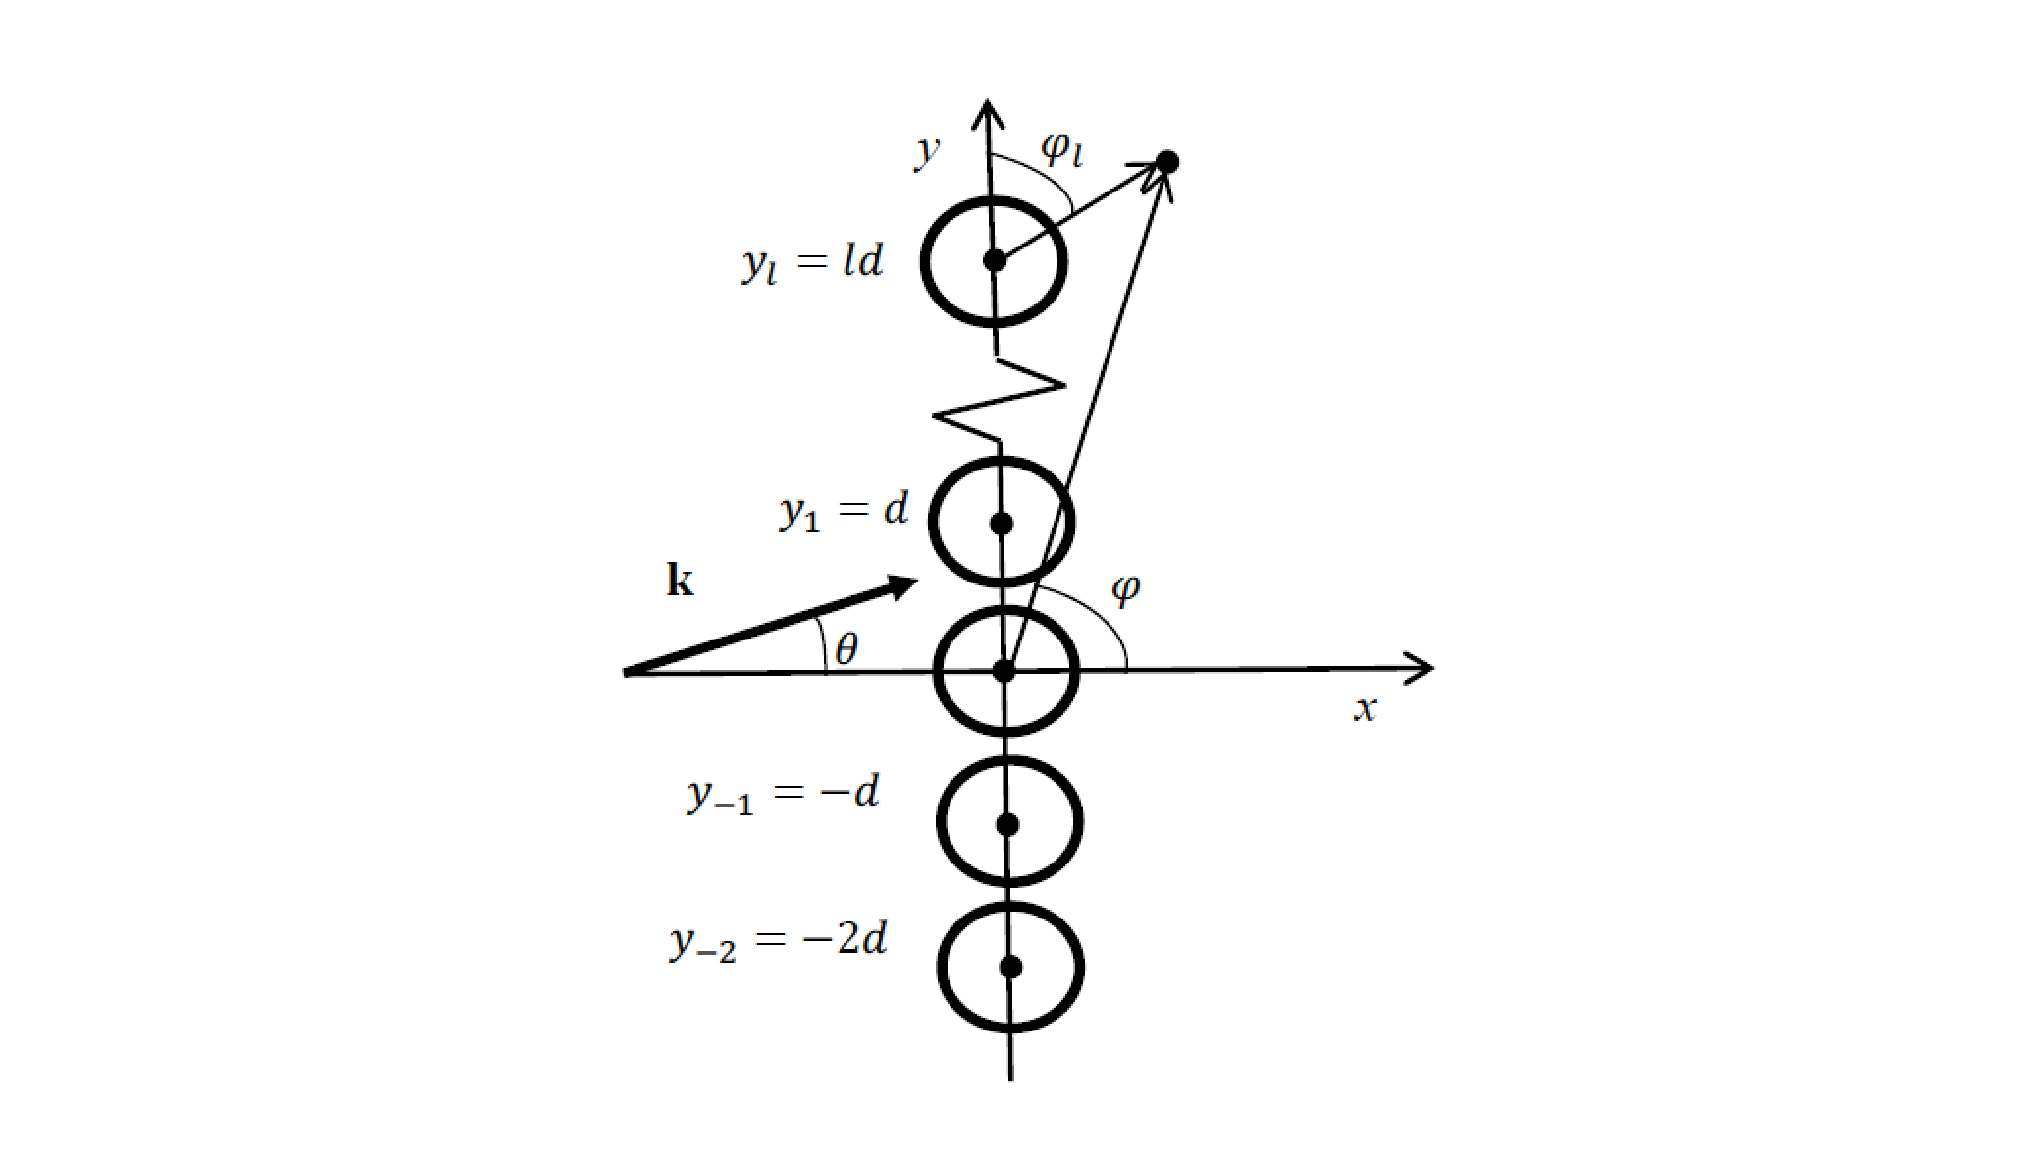
\includegraphics[width=\linewidth]{chaingeometry.eps}
\caption{Top view of the~perforated cylindrical shells aligned along the~$y$-axis with the~period $d$. Polar angles are shown for the~central ($l=0$) and $l$-th units. The~acoustic plane wave is incident at the~angle $\theta$ on the~chain.}
%The~Cartesian coordinates ${\bf r}=(x,y)$ are related to the~polar coordinates $(r_l,\varphi_l)$ associated with the~center of the~$l$-th cylinder: $x=r_l \cos\varphi_l$, $y=y_l + r_l \sin \varphi_l$.}%
\label{fig:geometryChain}
\end{center}
\end{figure}

I start with the~analysis of the~sound interaction with the~finite chain of $2N+1$ scatterers.
The~scatterers are spread along a~straight line, with their axes intersecting the~$y$-axis at the~points $y_n = nd$, $n=0,\pm1,\pm2,\dots, \pm N$ (see \cref{fig:geometryChain}).
The~neighboring shells are separated by a~distance $d=11.0$ cm, which serves as the~period of the~chain.
The~incoming sound is modeled by a~monochromatic plane wave which approaches from the~left at an~angle $\theta$.
Namely, the~pressure of the~incident wave is $p({\bf r},t)=p_0\exp(i{\bf k\cdot r} -i \omega t)$, where the~wave vector ${\bf k}$ has the~components of ${\bf k} = (k_x,k_y,0) = (k \cos\theta,k \sin\theta,0)$.

The~solution to the~scattering problem will be obtained for both finite and infinite chains of perforated shells.
The~latter only requires taking the~limit of $N\rightarrow\infty$, and allows for additional simplifications as the~Bloch theorem becomes applicable.
Similar problems were investigated in \cite{sainidou,zhang}.
The~two dealt with the~scattering of acoustic waves at a~periodic array of solid spheres in fluid and at a~monolayer of elastic spheres in air, respectively.
Also, such scattering problems are of interest in electrodynamics as well, namely, the~work \cite{vergeles} presented an~analysis of the~reflection of electromagnetic waves from an~infinite line of conducting cylinders.

In general, scattering of waves by an~infinite periodic array of cylinders constitutes one of the~classical problems in the~theory of diffraction.

%Scattering of waves by an~{\it infinite} periodic chain of cylinders is one of the~classical problems of theory of diffraction. For conducting cylinders illuminated by an~electromagnetic wave the~expansion of the~scattered field was proposed in \cite{vergeles}. For sound waves, the~field distribution resulting from diffraction in a~periodic array of solid spheres in fluid was calculated in \cite{zhang}. A~similar problem for elastic waves scattered by a~monolayer of elastic spheres was solved in \cite{sainidou}. In these studies, the~chain of scatterers was considered to be infinite, i.e., the~Bloch theorem was applicable. Here we first calculate the~acoustic field scattered by a~finite-length chain. A~periodic infinite chain is analyzed in the~next section.



\subsection{Scattered and Transmitted Pressure Fields}

Based on the~geometry of the~problem, it is convenient to develop the~solution in the~cylindrical coordinate system.
Each cylindrical shell will have a~separate coordinate system associated with it, and I will use the~notion of $(r_l,\varphi_l,z)$ for the~coordinates of a~point in space with respect to the~$l$-th coordinate system.
The~origin of each system is located at the~point $y_l=ld$, i.e., the~axis of each cylinder coincides with the~$z$-axis of the~respective coordinate system, as shown in \cref{fig:geometryChain}.

The~incoming pressure plane wave
\begin{equation}
p({{\bf r},t}) = p_0 \exp(i {\bf k \cdot r}-i \omega t)
\end{equation}
is represented in each of those coordinate systems by the~series
\begin{equation}
\label{eq:3Chain}
p({{\bf r},t})~=~{p}\left(r_l,\varphi_{l},t \right) = p_0 e^{i k r_l\cos\left(\varphi_l-\theta\right)-i \omega t}
~=~p_0\sum\limits_{n=-\infty}^{\infty}i^{n} J_{n}\left(k r_l\right) e^{i n\left(\varphi_l-\theta\right) -i \omega t}.
\end{equation}
where the~wave vector $k$ is $k=\omega/c_0$.
The~harmonic time dependence $e^{-i \omega t}$ will be omitted further below.

The~pressure field obeys the~wave equation \cref{eq:waveeqPRayleigh}, which in the~cylindrical coordinates is expressed as
\begin{equation}
\label{eq:waveeqPCylChain}
\frac{1}{r}\frac{\partial}{\partial r}\left(r\frac{\partial p}{\partial r}\right) + \frac{1}{r^2}\frac{\partial p}{\partial \varphi^2} + k^2 p(r,\varphi)~=~0.
\end{equation}
The~derivative with respect to $z$ does not appear above as the~problem is assumed to be uniform along $z$.
If the~angular dependence is eliminated by assuming the~proportional to $e^{in\varphi}$, $n=0,\pm1,\pm2,...$, behavior of pressure, then the~solutions of the~radial part of the~wave equation \cref{eq:waveeqPCylChain} are the~Bessel functions of the~order $n$.

This knowledge allows to write down the~acoustic field scattered by an~array of shells as a~superposition of cylindrical waves:
\begin{equation}
\label{eq:4Chain}
p_{sc}(r,\varphi) = \sum\limits_{l'} \sum\limits_{n=-\infty}^{+\infty} B_{l'n} H_{n}^{(1)}\left(k r_{l'}\right) e^{i n \varphi_{l'}}, \qquad r_l' \geq a.
\end{equation}
The~inner sum over $n$ represents the~total field radiated by each $l'$-th shell with respect to the~coordinate system aligned with that shell.
The~outer sum over $l'$ adds those contributions together to produce the~total scattered field.
The~value of $l'$ runs from $-N$ to $N$ for a~finite chain, or from $-\infty$ to $+\infty$ for an~infinite chain.
The~Hankel functions of the~first kind $H_n^{(1)}(kr)$ (or simply $H_n(kr)$) are chosen for the~expansion \cref{eq:4Chain} as they describe the~outgoing waves due to their asymptotic behavior $H_n^{(1)}(kr) \sim e^{ikr}/\sqrt{kr}$ at infinity.

The~use of multiple coordinate systems within the~same equation \cref{eq:4Chain} is perplexing and undesirable, and it is best to rewrite the~expression of the~scattered pressure field in terms of only the~coordinates $(r_l, \varphi_l)$ of the~certain $l$-th system.
Fortunately, since one has a~trivial relation between the~Cartesian coordinates ${\bf r}=(x,y)$ and the~polar coordinates $(r_l,\varphi_l)$ in the~form of 
\begin{align}
x~&=~r_l \cos\varphi_l, \\
y~&=~ld + r_l \sin \varphi_l,
\end{align}
then the~transformation between $(r_l,\varphi_l)$ and $(r_{l'},\varphi_{l'})$ is as follows:
\begin{align}
r_{l'} \cos\varphi_{l'}~&=~r_l \cos\varphi_l, \label{eq:5aChain} \\
r_{l'} \sin\varphi_{l'}~&=~(l-l')d + r_l \sin \varphi_l, \label{eq:5bChain}
\end{align}
For the~polar coordinates related by \cref{eq:5aChain}-\cref{eq:5bChain}, the~Graf's addition theorem (see Appendix \ref{appGrafTheorem}) applies:
\begin{equation}
\label{eq:6Chain}
H_{n}(k r_{l'}) e^{in \varphi_{l'}} = \sum\limits_{n'=-\infty}^{\infty}i^{(n+n') \sign(l-l')} H_{n+n'}(k |l-l'| d) J_{n'}(k r_l) e^{i n'(\pi- \varphi_l)},
\end{equation}
given that the~conditions $l' \neq l$ and $r_l<|l-l'|d$ are met.

As a~result, one arrives at the~expression for the~scattered field \cref{eq:4Chain} that involves only one pair of coordinates $(r_l, \varphi_l)$ and is valid for $r_l<d$, i.e., only in the~vicinity of the~$l$-th perforated shell:
\begin{align}
\label{eq:7Chain}
p_{sc}(r_l,\varphi_l) = \sum\limits_{n=-\infty}^{+\infty} \Bigg[&B_{ln} H_{n}\left(k r_l\right) e^{i n \varphi_l}+ \Bigg.\\
+\Bigg. &\sum\limits_{l' \neq l} B_{l'n}\sum\limits_{n'=-\infty}^{+\infty}i^{(n+n')\sign(l-l')}H_{n+n'}\left(k |l-l'| d\right) J_{n'}\left(k r_l\right) e^{i n'(\pi - \varphi_l)} \Bigg]. \notag
\end{align}
The~obtained expansion will prove extremely useful for the~purpose of dealing with the~boundary conditions at the~surfaces of the~shells.

As for the~pressure fields inside each $l$-th cylinder, I write their expansions over the~Bessel functions
\begin{equation}
\label{eq:8Chain}
p_{in}^{(l)}(r_l,\varphi_l) = \sum_{n=-\infty}^{\infty} {C_{ln} J_n(k r_l)e^{in \varphi_l}}, \qquad r_l \le b.
\end{equation}
All other cylinder functions are still valid solutions of the~wave equation \cref{eq:waveeqPCylChain}, but they cannot enter the~series \cref{eq:8Chain} as they diverge when $r_l\rightarrow 0$ and therefore do not describe any physically reasonable field behavior.



\subsection{Boundary Conditions at the~Surfaces of the~Shells}

As was discussed earlier, the~acoustic fields on either side of the~perforations are related in a~simplified fashion which, nevertheless, does not undermine the~resulting accuracy of calculations.
Namely, even though each perforated shell has a~finite thickness $h$, its value is much smaller than either of the~radii $a$ and $b$, and thus one can view the~two cylindrical faces of each shell as a~virtually single interface.
The~fluid-metal interactions are already encompassed inside the~effective impedance \cref{eq:ZpChain}, and one only needs to relate the~pressure fields outside the~shells with those inside the~shells.
 
The~condition \cref{eq:bcChain} prescribes to assume the~radial component of the~velocity of the~fluid (that is, normal to the~interface) to be unchanged across the~thickness of the~metal, and also relates it to the~pressure discontinuity between the~faces of the shells:
\begin{equation}
\label{eq:9Chain}
v_r|_{r=a} = v_r|_{r=b} = \dfrac{p|_{r=b} - p|_{r=a}}{Z_p}
\end{equation}

The~radial velocity in fluid is derived from the~local pressure according to \cref{eq:vandpRayleigh}:
\begin{equation}
\label{eq:10Chain}
v_r = \dfrac{1}{i\omega\rho_0}\dfrac{\partial p}{\partial r}.
\end{equation}

From the~three equations that appear in \cref{eq:9Chain}, I will be using the~following two independent relations:
\begin{align}
\label{eq:10aChain}
v_r|_{r=a}~&=~v_r|_{r=b}, \\
p|_{r=a}~&=~p|_{r=b}-Z_p v_r|_{r=b},
\end{align}
where the~place of the~pressure outside the~shell $p|_{r=a}$ will be taken by the~superposition of the~incoming and scattered waves $p+p_{sc}$, and the~pressure inside the~shell $p|_{r=b}$ is exactly the~pressure field $p_{in}^{(l)}$.

The~method of expressing the~acoustic fields in terms of series over cylinder functions and matching them via the~boundary conditions is exact since its solution is the~total \textit{true} field.
As opposed to this, the~approach based on the~$T$-matrix method and the~multiple scattering theory used in \cite{garcia2,garcia1} is only approximate as it discards the~high-order scatterings of the~waves.

The~dissipation of energy due to the~viscous effects in air is accounted for via the~effective impedance $Z_p$ of the~perforated shells.
The~viscous friction at the~air-metal interfaces is practically the~only reason for the~energy loss.
The~dissipation within the~bulk volume of air is almost nonexistent at the~frequencies of several kHz, the~typical decay length being on the~order of several kilometers.

Note that since the~elastic vibrations of the~metal are not considered explicitly in this approach, there is neither need nor advantage in using the~notion of acoustic potentials \cref{eq:waveeqBRayleigh,eq:waveeqLRayleigh,eq:waveeqSRayleigh} in solving this problem.


\section{Solution for the~Scattered Acoustic Field}

\subsection{Finite Chain of Perforated Shells}

The~equations \cref{eq:3Chain}, \cref{eq:7Chain}, and \cref{eq:8Chain} express the~pressure fields basically in the~form of Fourier expansions over $e^{in\varphi_l}$.
Because of that, the~angular dependence in the~boundary conditions \cref{eq:10Chain} can be eliminated by applying the~Fourier transform,
splitting each condition into a~set of equations for the~respective Fourier coefficients.
This results in the~following set of linear equations for the~unknowns $B_{ln}$ and $C_{ln}$:

\begin{equation}
\label{eq:11Chain}
\left\{
\begin{array}{rll}
C_{ln} \dfrac{J'_{n}\left(k b\right)}{J'_{n}\left(k a\right)}~&=~p_0 i^n e^{-i n\theta} &+ B_{ln} \dfrac{H'_{n}\left(k a\right)}{J'_{n}\left(k a\right)} + \\
& &+ \dsum\limits_{l' \neq l} \dsum\limits_{n'=-\infty}^{\infty} i^{(n-n')\sign(l-l')}H_{n-n'}(k|l-l'|)d) B_{l'n'},\\
 & & \\
%
%
\dfrac{i k Z_p}{\omega\rho_0}\,C_{ln} \dfrac{J'_{n}\left(k b\right)}{J_{n}\left(k a\right)} + C_{ln} \dfrac{J_{n}\left(k b\right)}{J_{n}\left(k a\right)}~&=~p_0 i^n e^{-i n\theta} &+ B_{ln} \dfrac{H_{n}\left(k a\right)}{J_n\left(k a\right)} + \\
& &+ \dsum\limits_{l' \neq l} \dsum\limits_{n'=-\infty}^{\infty} i^{(n-n')\sign(l-l')}H_{n-n'}(k|l-l'|)d) B_{l'n'}.\\
\end{array}
\right.
\end{equation}
The~index $n$ indicates which specific Fourier component the~equations are written for, and the~index $l$ enumerates the~shells, meaning that the~equations containing $C_{ln}$ resulted from applying the~boundary conditions to the~$l$-th shell.

The~scattered acoustic field depends only on the~unknown $B_{ln}$, so one may substitute the~value of $C_{ln}$ obtained from the~first row of \cref{eq:11Chain} into the~second row, and obtain the~system of linear inhomogeneous equations for $B_{ln}$ only:
\begin{equation}
\label{eq:12Chain}
\mathcal{S}_n B_{ln} + \sum\limits_{l' \neq l} \sum\limits_{n'=-\infty}^{\infty} i^{(n-n')\sign(l-l')} H_{n-n'}\Big(k|l-l'|d\Big) B_{l'n'} = -p_0 i^n e^{-i n\theta},
\end{equation}
where $\mathcal{S}_n$ denotes the~fraction
\begin{equation}
\label{eq:13Chain}
\mathcal{S}_n = \dfrac{H_n\left(k a\right)-H'_n\left(k a\right)\left(\dfrac{i Z_p}{\rho_0 c_0}+\dfrac{J_{n}\left(k b\right)}{J'_{n}\left(k b\right)}\right)}{J_n\left(k a\right)-J'_n\left(k a\right)\left(\dfrac{i Z_p}{\rho_0 c_0}+\dfrac{J_{n}\left(k b\right)}{J'_{n}\left(k b\right)}\right)}.
\end{equation}
The~last step in calculating the~distribution of the~scattered field \cref{eq:4Chain} from a~finite chain of perforated shells is solving the~linear set \cref{eq:12Chain}, which will be done numerically.


\subsection{Infinite Chain of Perforated Shells}

For an~infinite periodic chain of scatterers ($N=\infty$), the~obtained system \cref{eq:12Chain} still remains valid.
Moreover, it can be now further simplified since it is imperative to benefit from the~established periodicity of the~system along the~$y$-axis.
The~Bloch theorem guarantees that in a~periodic environment a~propagating wave $\psi(x,y)$ is represented as $\psi(x,y)~=~e^{iqy}\upsilon(x,y)$, where the~function $\upsilon(x,y)$ is periodic, $\upsilon(x,y)=\upsilon(x,y+d)$, and $q$ is the~$y$-component of the~ wavevector of the~wave.

The~incident at the~chain plane wave determines the~wavevector $q$:
\begin{equation}
q~=~k_y~=~k\sin\theta,
\end{equation}
and to satisfy the~inferences of the~Bloch theorem, the~unknown amplitudes $B_{ln}$ must be related to the~values $B_{0n}$ associated with the~shell in the~middle of the~chain:
\begin{equation}
\label{eq:14Chain}
B_{ln} = e^{ik_yld} B_{0n}.
\end{equation}
I substitute the~latter relation into \cref{eq:12Chain}, redefine the~unknowns as $b_n=i^{-n}B_{0n}$, and arrive at the~following set of linear equations:
\begin{equation}
\label{eq:15Chain}
\mathcal{S}_n b_{n} + \sum\limits_{n'=-\infty}^{\infty} F(n'-n) b_n' = -p_0 e^{-i n\theta}, \,\, n=0,\pm1,\pm2,\dots
\end{equation}
Here the~lattice sum $F(n)$ is an~infinite series
\begin{equation}
\label{eq:latticesum}
F(n)= \sum\limits_{l'=1}^{+\infty} H_{n}\left(k l'd\right) \left[e^{i k_y l' d} + (-1)^{n} e^{-i k_y l' d}\right],
\end{equation}
the~calculation of which is discussed in Appendix \ref{appConvSeries}.

A~similar set of equations was obtained in \cite{vergeles,evans} for scattering of waves at an~infinite periodic chain of metallic cylinders.




\section{Eigenmodes of an~Infinite Chain of Scatterers}


\subsection{Dispersion Relation}

\begin{figure}
\begin{center}
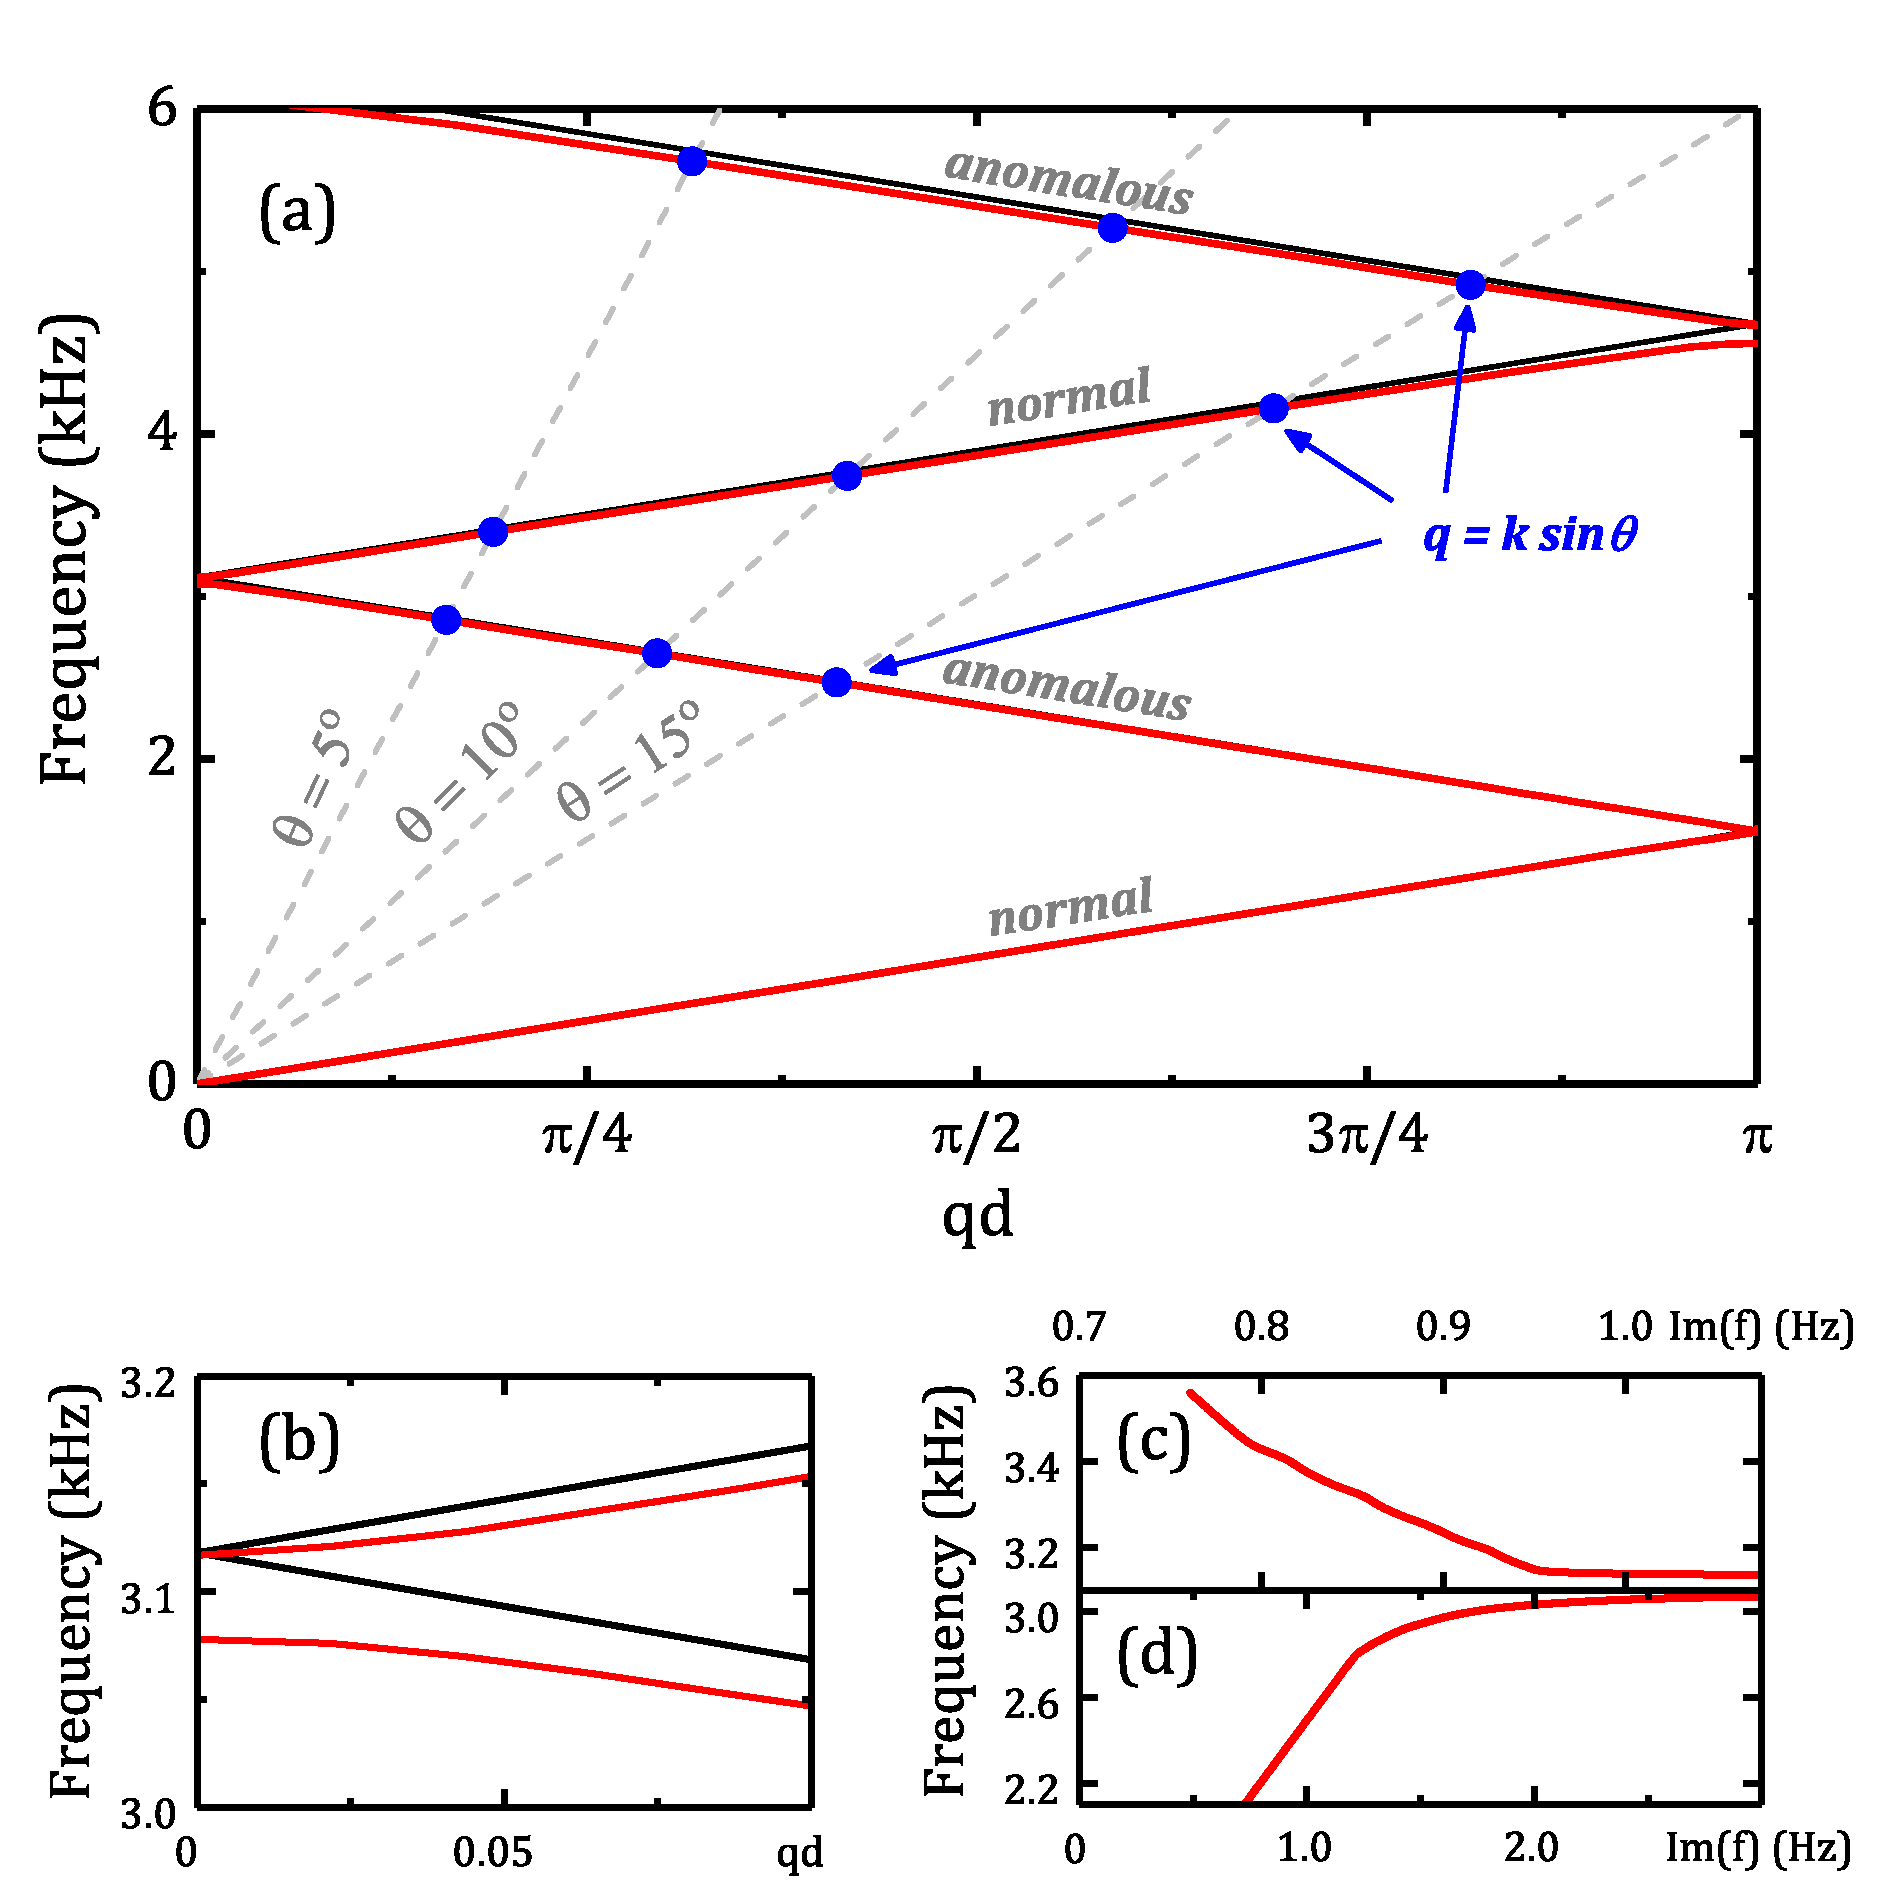
\includegraphics [width=0.9\linewidth]{dispChain.eps}
\caption{(a) Band structure of an~infinite periodic chain of shells in inviscid air environment. Straight black lines show linear dispersion in air. Red lines are the~real parts of eigenfrequencies calculated from \cref{eq:17Chain}. Crossings of the~dispersion curves with three dashed straight lines \cref{eq:18Chain} give the~frequencies of resonant coupling of the~incident plane wave to the~eigenmodes of the~chain for three angles of incidence, $\theta = 5^{\circ}$, $\theta = 10^{\circ}$, and $\theta = 15^{\circ}$. (b) Band splitting at the~$\Gamma$-point near the~frequency $f=3.1$ kHz; the~distance between the~levels in the~doublet is 35 Hz. (c),(d) Absolute value of the~imaginary part of eigenfrequency vs its real part for the~region near 3.1 kHz.}
\label{fig:dispChain}
\end{center}
\end{figure}
%\textcolor{red}{The~Wood's anomalies are observed at these resonant frequencies.}  The~horizontal axes, where the~imaginary part of the~frequency is plot, are different for the~upper and lower levels of the~doublet. 

Here I analyze the~eigenmodes that can be supported by the~infinite chain of perforated shells in order to gain additional insights about its capability to suppress sound transmission.
The~eigenmodes are the~waves propagating in either direction along the~chain and are characterized by the~wavevector $q$.
They are the~nontrivial solutions of \cref{eq:15Chain}, in which the~right-hand side contains no incident wave.
By equating the~determinant of a~corresponding homogeneous linear system to zero,
\begin{equation}
\label{eq:17Chain}
\det |\mathcal{S}_n \delta_{nn'} + F(n'-n)|=0,
\end{equation}
one obtains the~equation that defines the~dispersion relation $\omega=\omega(q)$ of the~eigenmodes.

Finding the~solution to \cref{eq:17Chain} is complicated by the~necessity to calculate the~determinant of an~infinite matrix and by having to deal with the~slow-converging series \cref{eq:latticesum}.
The~latter issue is addressed by identically replacing $F(n)$ with the~fast-converging series originally found in \cite{twersky} and subsequently used in \cite{vergeles, evans} (see Appendix \ref{appConvSeries}).

\cref{fig:dispChain}(a) visualizes the~few lowest bands of the~dispersion equation, which are calculated numerically.
Due to perforated shells being weak scatterers, the~resulting dispersion curve (shown in red) is almost identical to the~band structure describing the~empty-lattice model (shown in black).
The~differences between the~two appear only near the~$\Gamma$-point $q=0$ (and also at the~zone edge $q=\pi/d$), where the~level doublet is formed due to the~level repulsion, forming a~gap.
The~gap size is approximately $35$ Hz between the~second and the~third bands (which is near the~frequency of $3.1$ kHz).
The~first (lowest) band and other odd-numbered bands have normal dispersion, whereas every even-numbered band exhibits anomalous dispersion.
As can be seen in \cref{fig:dispChain}(b), the~dispersion of the~bands becomes essentially nonlinear towards the~$\Gamma$-point.

It is also peculiar that the~two bands of the~doublet exhibit different behavior: only for the~lower band does the~group velocity vanish when $q=0$, thus making the~gap opening strongly asymmetric.
Moreover, the~upper band exhibits a~singularity which is not resolved in \cref{fig:dispChain}.
The~behavior of both bands will be analyzed in more detail further in this chapter.

The~solutions $\omega(q)=2 \pi f(q)$ of the~transcendental dispersion equation \cref{eq:15Chain}, found for real values of the~wave vector $q$, are complex.
This makes the~acoustic eigenmodes of an~infinite chain leaky, regardless of whether the~viscosity of the~fluid is accounted for.
Leaky eigenmodes are not strongly localized in the~vicinity of the~chain, instead they carry the~acoustic energy away from it, and the~imaginary part of the~frequency describes the~strength of radiative decay.

Nevertheless, the~leaky modes may still be long-living excitations if the~decay is very slow, i.e., if the~imaginary part $\im f$ is small.
As is shown in \cref{fig:dispChain}(c,d), the~rate of radiative decay $|\im f|$ is smaller than the~frequency of sound $f \approx \re f$ by at least two orders of magnitude.
Namely, near the~$\Gamma$-point this rate is about $1$-$3$ Hz, which practically does not affect the~width of the~resonance minima in the~transmission spectra, as will be discussed below.
The~use of the~absolute value to characterize the~decay rate $|\im f|$ indicates that the~imaginary part of frequency is negative, $\im f < 0$, which is imperative in order to have the~time-dependent term $e^{-i\omega t}$ exponentially decreasing and not increasing with time.

%The~numerical solution of this dispersion equation for the~few lowest bands is presented in \cref{fig:dispChain}. Since perforated shells are weak scatterers, the~dispersion curve (blue dots) is very close to the~band structure obtained in the~empty-lattice model, shown by the~straight broken line (red). Only at the~$\Gamma$-point $q=0$ (and at the~edge $q=\pi/d$) the~effect of level repulsion leads to gap opening of 35 Hz and essentially nonlinear dispersion, see the~left insert to \cref{fig:dispChain}. It is shown in Appendix B \textcolor{red}{!!!} that near the~point of degeneracy, $f = 3078$ Hz, the~upper and lower bands exhibit different behavior. In particular, the~gap opening is strongly asymmetric and the~group velocity vanishes at $q=0$ only for the~lower band. There are also some singularities in the~dispersion of the~upper band which are not resolved in \cref{fig:dispChain}. They are shown in the~insert to \cref{fig:asymgapChain}.  Away from the~$\Gamma$-point the~dispersion of the~both bands is practically linear but it is normal for the~upper band and anomalous for the~lower one.

%For real values of the~wavevector $q$ all the~solutions $\omega(q)=2 \pi f(q)$ of the~transcendental equation \cref{eq:15Chain} are complex. This means that the~acoustic eigenmodes of an~infinite chain of shells are leaky modes, even if the~viscosity of the~fluid is neglected. The~imaginary part of frequency describes weak radiative decay, i.e., the~acoustic eigenmodes are not strongly localized near the~chain.

%However, since the~decay is very slow the~leaky eigenmodes are long-living excitations. The~imaginary part is negative, $\text{Im }f<0$, in order for the~time-dependent factor $e^{-i\omega t}$ to decay with time. The~rate of radiative decay $|\text{Im }f|$ is at least two orders of magnitude smaller than the~frequency of sound $f \approx \text{Re }f$ as it can be seen from the~right insert to \cref{fig:dispChain}. For the~frequencies near the~$\Gamma$-point the~rate of radiative decay is about 1-3 Hz, i.e., it practically does not contribute to the~width of the~resonance minima as will be shown below.



\subsection{Analysis of the~Asymmetric Band Gap}

Here I will analyze the~behavior of the~two bands forming a~doublet near the~$\Gamma$-point (see \cref{fig:dispChain}(c)).
This can be done using an~approach that treats the~perforated shells as a~small perturbation to the~uniform air background.
In zero approximation, i.e., in the~empty-lattice model, the~dispersion bands are linear.
When the~small perturbations are introduced, the~differences between the~linear bands and the~actual dispersion curves found by solving \cref{eq:17Chain} are small, and are only significant in the~vicinity of the~$\Gamma$-point and the~edges of the~Brillouin zone, i.e., only near the~points of degeneracy.
In the~theory of band structures, the~perturbation theory for degenerate states is typically used to calculate such band corrections.
However, the~degeneracy is removed from the~picture by the~presence of weak scattering, and the~narrow band gaps are formed.
In solids, applying such perturbation theory results in the~so-called nearly free electron model, where the~unperturbed eigenfunctions are represented by a~basis of simple plane waves.
In the~case of a~chain of perforated shells, the~basis of cylindrical functions needs to be used, and thus the~perturbation theory that will apply here will strongly differ from that in the~nearly free electron model.
Even though the~final result --- forming of narrow band gaps --- is expected to be qualitatively the~same, I will still obtain the~explicit expressions for the~level repulsion near the~points of degeneracy and compare obtained formulas with the~values found by solving the~exact dispersion equation \cref{eq:17Chain} numerically.
I will show that the~strength of the~level repulsion is essentially different from what is known in the~nearly free electron model.
The~reason behind this is the~specific form of the~boundary condition \cref{eq:9Chain}, which approximates the~interaction of the~shell with the~background using the~impedance approach and assumes a~discontinuity of pressure on the~two surfaces of the~shell even for very thin shells.

%Assuming that the~perforated shells are weak scatterers, the~solution of the~dispersion equation \cref{eq:17Chain} can be found using a~perturbation theory. In zero approximation, the~dispersion that corresponds to the~empty-lattice model is linear. Corrections to this linear dispersion are of interest only near the~points of degeneracy, i.e., in the~vicinity of the~$\Gamma$-point and the~edges of the~Brillouin zone.
%In the~theory of band structures, these corrections are usually obtained using perturbation theory for degenerate states. Due to weak scattering, the~degeneracy is lifted, giving rise to narrow band gaps. In solids, this kind of perturbation theory is known as the~nearly free electron model and it uses the~basis of plane waves as unperturbed eigenfunctions. Here we look for the~solution of the~wave equation in the~basis of cylindrical functions that leads to strong modification of the~perturbation theory as compared to the~well-known nearly free electron model.
%While the~final result is the~same -- opening of narrow band gaps, it is worthwhile to get the~explicit formulas for the~gap width and for the~level repulsion near the~points of degeneracy and to compare these formulas with the~results obtained nonperturbatively from the~exact dispersion equation \cref{eq:17Chain}. It will be shown that because of the~specific form of the~boundary condition \cref{eq:9Chain}, which assumes a~discontinuity of pressure even for very thin shell, the~strength of the~level repulsion is quite different from that observed in the~nearly free electron model.

%The~numerical solution of the~dispersion equation \cref{eq:17Chain} showed that the~dispersion of the~chain eigenmodes is linear everywhere except , where the~level repulsion leads to parabolic dispersion.
%\begin{equation}
%\label{B1}
%\det |\mathcal{S}_n \delta_{nn'} + F(n'-n)|=0
%\end{equation}
%Moreover, this solution must become identical to the~empty-lattice model dispersion when there are no shells, which corresponds to the~limit of %vanishing thickness of the~shells, $h = (a - b) \rightarrow 0$, and vanishing impedance, $Z_p \rightarrow 0$.
%Here we develop a~perturbation theory for the~band structure calculation which is formally equivalent to the~nearly free electron model in solids. to find the~analytical solution of the~dispersion equation \cref{eq:17Chain}, where the

The~absence of the~perforated shells, which implies no scattering of sound, can be obtained by decreasing the~acoustic impedance to zero, $Z_p\rightarrow 0$.
This fact makes it different from the~situation where the~absence of scattering from a~solid cylinder is normally realized by matching the~impedances $\rho c$ of the~background fluid and the~cylinder.
The~parameter $Z_p$ will serve as a~small perturbation in the~perturbation theory.
The~smallness of $Z_p$ also requires the~shells to be extremely thin, $h=\left(a-b\right) \rightarrow 0$, however, the~thickness cannot be used as a~small parameter as the~latter condition only is not sufficient itself (see \cref{eq:ZpChain} and \cref{eq:ZpIdealChain}).


%The~scattering of sound by perforated cylinders vanishes when the~acoustic impedance $Z_p\rightarrow 0$. This situation is different from the~case of solid cylinders when absence of scattering requires matching of the~impedance of the~material of the~cylinders and the~impedance $c_0\rho_0$ of the~background fluid.  Thus, the~small parameter of the~perturbation theory is impedance $Z_p$ that requires that the~thickness of the~shell $h=\left(a-b\right) \rightarrow 0$. The~latter condition is necessary but not sufficient, as it is seen from Eqs. \cref{1} and \cref{2}.

The~coefficient $\mathcal{S}_n$ in \cref{eq:13Chain} approaches infinity when $a\rightarrow b$ and $Z_p \rightarrow 0$, which allows rewriting the~dispersion relation \cref{eq:17Chain} in the~following form:
\begin{equation}
\label{eq:B3Chain}
\det \left|\delta_{nn'} + \dfrac{F(n'-n)}{\mathcal{S}_n}\right|=0.
\end{equation}
Since $F(n'-n)/\mathcal{S}_n \ll 1$, the~matrix in \cref{eq:B3Chain} is almost diagonal and its determinant can be approximated by
\begin{equation}
\label{eq:B4Chain}
\det \left|\delta_{nn'} + \dfrac{F(n'-n)}{\mathcal{S}_n}\right| \approx \det |\delta_{nn'}| + \Tr\left( \dfrac{F(n'-n)}{\mathcal{S}_n}\right)
= 1 + F(0)\sum_{n=-\infty}^{+\infty}\mathcal{S}_n^{-1}.
\end{equation}
I further expand the~terms $\mathcal{S}_n^{-1}$ in the~series \cref{eq:B4Chain} over the~small parameters $h=a-b$ and $Z_p$.
In the~linear approximation one arrives at the~expression
\begin{align}
\label{eq:B5Chain}
\mathcal{S}_n^{-1} &= \dfrac{J_n\left(k a\right)-J'_n\left(k a\right)\left(\dfrac{i Z_p}{\rho_0 c_0}+\dfrac{J_{n}\left(k b\right)}{J'_{n}\left(k b\right)}\right)}{H_n\left(k a\right)-H'_n\left(k a\right)\left(\dfrac{i Z_p}{\rho_0 c_0}+\dfrac{J_{n}\left(k b\right)}{J'_{n}\left(k b\right)}\right)} = \\
%
&= \dfrac{-\dfrac{i Z_p}{\rho_0 c_0} J'_{n}\left(k a\right)J'_{n}\left(k b\right) + \Big(J_n\left(k a\right)J'_{n}\left(k b\right)-J'_n\left(k a\right)J_{n}\left(k b\right)\Big)}{-\dfrac{i Z_p}{\rho_0 c_0} J'_{n}\left(k a\right)J'_{n}\left(k b\right) + \Big(H_n\left(k a\right)J'_{n}\left(k b\right)-H'_n\left(k a\right)J_{n}\left(k b\right)\Big)} \approx \notag\\
%
&\approx \dfrac{-\dfrac{i Z_p}{\rho_0 c_0} J'^{2}_{n}\left(k a\right) + k(b-a)\Big(J_n\left(k a\right)J''_{n}\left(k a\right)-J'_n\left(k a\right)J'_{n}\left(k a\right)\Big)}{H_n\left(k a\right)J'_{n}\left(k a\right)-H'_n\left(k a\right)J_{n}\left(k a\right)} = \notag \\
%
&= \dfrac{-\dfrac{i Z_p}{\rho_0 c_0} J'^{2}_{n}\left(k a\right) + k(a-b)\Big(J'^2_n\left(k a\right)-J_n\left(k a\right)J''_{n}\left(k a\right)\Big)}{-\dfrac{2i}{\pi k a}} \approx \notag \\
%
&\approx \dfrac{\pi k a}{2i}\dfrac{i Z_p}{\rho_0 c_0} J'^{2}_{n}\left(k a\right) - \dfrac{1}{2i} \pi k^2 a(a-b) \Big(J'^2_n\left(k a\right)-J_n\left(k a\right)J''_{n}\left(k a\right)\Big). \notag
\end{align}
As is seen from \cref{eq:B5Chain}, the~expansion goes over two dimensionless parameters, $z~=~\dfrac{\pi k a}{2}\dfrac{i Z_p}{\rho_0 c_0}$ and
$\epsilon = \pi k^2 a h$.
Here $k=\omega/c_0$, so these parameters are real if the~background fluid is inviscid.
Since the~impedance $Z_p \propto \omega$ (see \cref{eq:ZpChain}), it follows that $z,\epsilon \propto \omega^2$ as well.
Such quadratic growth invalidates the~approximation \cref{eq:B5Chain} at high frequencies.

After the~expansion \cref{eq:B5Chain} is substituted into the~sum over $n$ in \cref{eq:B4Chain}, one obtains the~following result:
\begin{align}
\label{eq:B6Chain}
\sum_{n=-\infty}^{+\infty}\mathcal{S}_n^{-1} &= \dfrac{\pi k a}{2i}\dfrac{i Z_p}{\rho_0 c_0} \sum_{n=-\infty}^{+\infty} J'^{2}_{n}\left(k a\right) - \dfrac{1}{2i} \pi k^2 a h \sum_{n=-\infty}^{+\infty} \Big(J'^2_n\left(k a\right)-J_n\left(k a\right)J''_{n}\left(k a\right)\Big) = \notag \\
&= \dfrac{\pi k a}{4i}\dfrac{i Z_p}{\rho_0 c_0} - \dfrac{1}{2i} \pi k^2 a h = \frac{z - \epsilon}{2i}.
\end{align}
The~identities $\dsum_{n=-\infty}^{+\infty} J'^2_n(x) = -\dsum_{n=-\infty}^{+\infty} J_n(x) J''_n(x)=\frac12$ were employed here to simplify the~latter expression.
I finally rewrite \cref{eq:B3Chain} and \cref{eq:B4Chain} as
\begin{equation}
\label{eq:BB7Chain}
\frac{1}{F(0)} = -\sum_{n=-\infty}^{+\infty}\mathcal{S}_n^{-1} = -\frac{z - \epsilon}{2i}.
%= i\left(-\dfrac{\pi k a}{4}\dfrac{i Z_p}{\rho_0 c_0} + \dfrac12 \pi k^2 a (a-b)\right)^{-1}.
\end{equation}


In zero approximation, the~right-hand side of \cref{eq:BB7Chain} vanishes, and the~dispersion is thus obtained from the~condition $F(0)= \infty$.
In order to satisfy this condition, one of the~resonant terms with $\gamma_m= -i \sqrt{k^2 - q_m^2}$ in the~denominator in \cref{eq:latticesum1C} must become infinity as well.
The~divergence of any of these terms is achieved if their denominator is equal to 0, which leads to the~condition
\begin{equation}
\label{eq:B0Chain}
\omega=c_0\,| q \pm 2\pi m/d |, \,\,\, m=0,1,2,\dots.
 \end{equation}
The~obtained dispersion relation is exactly the~linear dispersion for sound in the~empty lattice approximation.

In the~first (linear) approximation over $z$ and $\epsilon$, the~same resonant terms need to remain in the~lattice sum:
\begin{equation}
\label{eq:BF1Chain}
F(0) \approx -\sum_{m=-\infty}^{\infty} \frac{2i}{\gamma_m d} \approx \frac{2}{d} \sum_{m=-\infty}^{\infty} \frac{1}{\sqrt{k^2 - (q + 2\pi m/d)^2}}.
\end{equation}
Since I am analyzing the~level splitting near the~$\Gamma$-point, it is convenient to represent the~parameter $k=\omega/c_0$ as $k = 2\pi m/d +\Delta k_m $, where $\Delta k_m$ is a~small correction.

As was already established, the~eigenmodes of the~chain of perforated shells are leaky waves, and the~numerically calculated dispersion bands $f(q)$ shown in \cref{fig:dispChain} contain small negative imaginary part which causes the~exponential decay of the~signal intensity with time $t \rightarrow \infty$.
However, evaluating the~function $F(n)$ (see \cref{eq:latticesum}) for the~values of $k$ from the~lower complex plane shows that the~function is singular, which is due to the~diverging sum of the~Hankel functions of the~complex argument.
Indeed, since the~Hankel function of the~first kind asymptotically behaves as $H_n(kl'd) \approx \sqrt{2/(\pi kl'd)} \exp(ikl'd - i\pi n/2 - i\pi/4)$, and if $k$ has any negative imaginary part, the~exponential term will grow infinitely with $l'$.
This issue is addressed in Appendix \ref{appConvSeries} by means of analytical continuation of the~function $F(n)$ into the~region $\im k < 0$.
The~function $F(n)$ can further be replaced by the~fast convergent series \cref{eq:latticesum1C}-\cref{eq:latticesum3C}, with the~only condition that one specifies which branch of $\sqrt{k^2-q_m^2}$ is to be used.

%At the~same time, the~function $F(n)$ defined by \cref{16} becomes singular in the~lower complex $k$ plane since the~sum over $l'$ diverges when the~complex argument of the~Hankel function infinitely grows.
%This follows from the~asymptotical behavior $H_n(kl'd) \approx \sqrt{2/(\pi kl'd)} \exp(ikl'd - i\pi n/2 - i\pi/4)$. The~function $F(n)$ can be analytically continued to the~region $\im k < 0$ by fast convergent series \cref{A2}-\cref{A4}, provided that a~single-valued branch of $\sqrt{k^2-q_m^2}$ is defined.

As is elaborated in Appendix \ref{appBranchCut}, the~branch cut defining how to calculate the~complex square root function should be chosen along the~negative imaginary axis, in order to guarantee the~correct behavior for propagating, leaky, and nonradiative waves.
However, the~latter argument was developed for the~case of plane waves having spatial dependence $e^{ik_xx+ik_zz}$, and thus is not immediately applicable to the~scattered sound expanded over cylindrical waves.
Still, one may consider the~acoustic field far away from the~chain, where it can be expanded over the~plane waves with the~parallel to the~chain wave vector components $q_m$ and perpendicular to the~chain components $\gamma_m = \sqrt{k^2-q_m^2}$.
Consequently, if using the~branch cut along the~negative imaginary axis in $\sqrt{k^2-q_m^2}$ provides the~correct physical behavior of all waves in the~expansion over plane waves, then this correct behavior is preserved after switching from the~basis of plane waves to cylindrical waves.

%While the~expansion of the~scattered field \cref{eq:7Chain} runs over cylindrical waves, the~parameter $\gamma_m = \sqrt{k^2-q_m^2}$ serves (far away from the~chain) as a~perpendicular to the~chain component of the~wave vector. A~leaky mode with $\re(k^2-q_m^2) >0$ and $\im (k^2-q_m^2) <0$ (fourth quadrant) radiates towards $x>0$.  The~corresponding exponent $e^{i\gamma_m x}$ oscillates with exponentially growing amplitude, i.e., $\re\gamma_m>0$ and $\im \gamma_m<0$ (fourth quadrant). Increase of the~amplitude "compensates" exponential decay of the~energy of leaky mode along the~direction of propagation \cite{lim,ingerbrigsten,maradudin1}. For the~square root $\sqrt{k^2-q_m^2}$ with its argument $k^2-q_m^2$ lying in the~forth quadrant, the~branch of the~square root lying also in the~same quadrant is defined if the~cut is made, e.g., along the~negative imaginary axis. This choice is made, among other options, because it also provides the~correct behavior for the~non-radiative (true) eigenmodes \cite{maradudin2,maradudin3}. Indeed, for the~non-radiative wave $\im k < 0$ and $\re\left(k^2-q_m^2\right) < 0$, so $\left(k^2-q_m^2\right)$ lies in the~third quadrant. Then its square root lies either in the~second or fourth quadrant. The~non-radiative condition requires that $\im \sqrt{k^2-q_m^2} > 0$. This condition uniquely defines the~branch of the~square root in the~second quadrant and the~branch cut along the~negative imaginary axis.

Now, with the~uniquely defined branch for $\gamma_m$ one can solve the~dispersion equation \cref{eq:BB7Chain} with $F(0)$ in the~form \cref{eq:BF1Chain}.
For any band in the~band structure enumerated by the~index $m$, one can omit all the~terms in the~sum in \cref{eq:BF1Chain} except for the~two with $m'=m$ and $m'=-m$ in order to calculate the~level repulsion near the~$\Gamma$-point.
Note that if the~repulsion is to be calculated near the~edge of the~Brillouin zone, one must keep the~terms with $m'=m$ and $m'=-m-1$, which give the~principal contribution.
In the~region near the~band gap opening at the~$\Gamma$-point, where $k = \omega/c_0 \approx 2\pi m/d$ and $q \ll \pi/d$, it is possible to simplify the~denominators in \cref{eq:BF1Chain} to $\sqrt{k^2- q_{\pm m}^2} \approx \sqrt{(4\pi m/d)(\Delta k_m \mp q)}$.
The~dispersion equation then takes the~following form in the~linear approximation:
\begin{equation}
\label{eq:B15Chain}
\frac{1}{\sqrt{\Delta k_m - q}} + \frac{1}{\sqrt{\Delta k_m + q}} = -i\sqrt{4\pi m d}\left(z - \epsilon\right)^{-1}.
\end{equation}

Obviously, only when both terms in the~left-hand side are purely imaginary does this equation have a~unique solution.
Since the~value of $q$ is assumed to be positive, one must require that $\Delta k_m < 0$ and also $|\Delta k_m| > q$.
Negative values of $\Delta k_m$ describe the~{\it lower branch} of the~dispersion curve near the~frequency $\omega = 2 \pi m c_0/d$.
The~equation for $\Delta k_m$ can further be rewritten as
\begin{equation}
\label{eq:BDChain}
\sqrt{|\Delta k_m| +q} + \sqrt{|\Delta k_m| - q} = 2 \sqrt{\frac{\Delta k_m^2 - q^2}{\kappa_m}},
\end{equation}
where $\kappa_m = (z-\epsilon)^2/\pi m d$.
This equation is valid for any value of the~Bloch vector $0 < q < |\Delta k_m|$.
I will solve this equation in the~close vicinity of the~$\Gamma$-point, where $q \ll |\Delta k_m|$, as it is sufficient for calculations of the~band gap width and the~qualitative behavior of the~dispersion branch.
It immediately follows from \cref{eq:BDChain} that $\Delta k_m(q=0) = \kappa_m$, which gives the~level shift at the~$\Gamma$-point.
If the~both parts of \cref{eq:BDChain} are expanded in series over $q$ up to the~quadratic terms, one obtains a~quadratic equation for $|\Delta k_m|$.
This equation has two solutions, but only the~one which is physically meaningful must be chosen:
\begin{equation}
\label{eq:BEChain}
\Delta k_m= -\kappa_m - \frac{3 q^2}{4 \kappa_m}.
\end{equation}
Based on this result, I arrive at the~dispersion relation for the~lower branch of the~doublet:
\begin{equation}
\label{eq:BFChain}
\omega(q)=\frac{2 \pi m c_0}{d}+ \Delta k_m c_0 \approx \frac{2 \pi m c_0}{d} -\kappa_m c_0 - \frac{3 q^2}{4 \kappa_m} c_0.
\end{equation}
This dispersion relation possesses all the~same properties as the~one in the~nearly free electron approximation.
Specifically, at the~$\Gamma$-point the~group velocity vanishes, the~band gap is formed due to the~red shift of the~eigenfrequency, and its width is proportional to the~square of the~perturbation parameter, $\kappa_m c_0 \propto (z-\epsilon)^2$.
The~obtained dispersion relation appears to be purely real and satisfying the~nonradiative condition $k^2-q_{\pm m}^2 < 0$.
The~imaginary part of the~spectrum is recovered when the~sum \cref{eq:BF1Chain} is approximated more accurately by keeping the~terms with $|m'| \neq m$.



\begin{figure}
\begin{center}
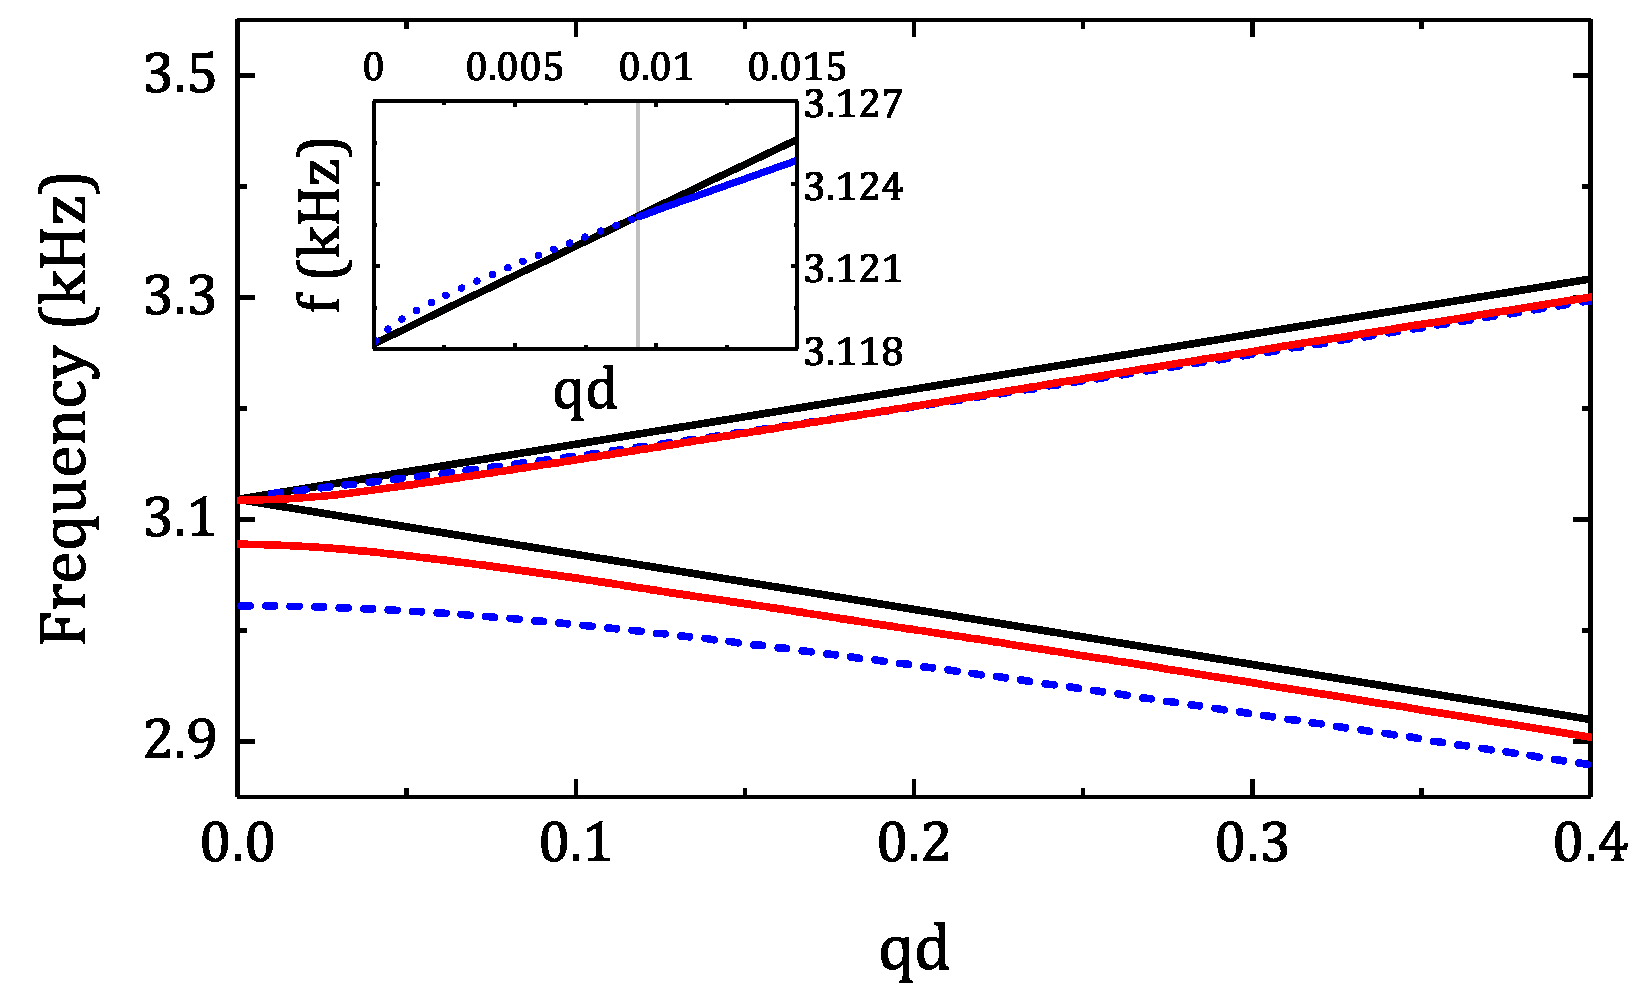
\includegraphics[width=0.8\linewidth]{asym_bandgap.eps}
\caption{Band structure of an~infinite periodic chain of shells in inviscid air environment. Solid black and red lines respectively show linear dispersion in air and dispersion calculated from \cref{eq:17Chain} (same as in \cref{fig:dispChain} (a)). Dashed blue lines show the~dispersion obtained from the~perturbation theory equations \cref{eq:BFChain} and \cref{eq:BGChain}. The~inset shows the~narrow region  $qd<q_cd \approx 0.01$ near the~$\Gamma$-point where the~upper band does not exist. The~leaky upper mode beyond $q=q_c$ is shown by blue line.}
\label{fig:asymgapChain}
\end{center}
\end{figure}


As for the~{\it upper} branch of the~dispersion curve, one may not treat $\Delta k_m$ as a~purely real value, so a~complex solution of \cref{eq:B15Chain} has to be found.
Since the~exponential decay with time is expected for all complex solutions, the~solution is restricted to the~lower part of the~complex plane, where $\im \Delta k_m = \im \omega/c_0 <0$.
However, the~right-hand-side of \cref{eq:B15Chain} remains to be purely imaginary, and therefore the~real parts of $(\Delta k_m - q)$ and $(\Delta k_m + q)$ need to have opposite signs.
This implies that the~term $(\Delta k_m - q)$ must lie in the~third quadrant, and the~term $(\Delta k_m + q)$ --- in the~fourth quadrant.
Because of that the~two inequalities $\re(\Delta k_m +q)>0$ and $\re(\Delta k_m -q)>0$ must be valid, which is achieved provided $|\re\Delta k_m| < q$.
The~latter condition cannot be satisfied when $q=0$, hence the~upper band never reaches the~$\Gamma$-point.
In \cref{eq:B15Chain}, the~first and the~second terms belong to the~third and the~first quandrants, respectively, given the~chosen branch cut along the~negative imaginary axis.
With that, I rewrite the~dispersion equation \cref{eq:B15Chain} using the~dimensionless variables $x=q/\kappa_m$ and $y= \Delta k_m/\kappa_m$ as
\begin{equation}
\label{eq:B16Chain}
\frac{1}{\sqrt{y-x}} = - 2i - \frac{1}{\sqrt{y+x}}.
\end{equation}
This equation can be squared and brought to a~biquadratic form over $x$, as both its left- and right-hand sides lie in the~same (third) quadrant.
After executing the~transformation mentioned one obtains:
\begin{equation}
\label{eq:B17Chain}
4 x^4 + x^2(1-8y^2-4y) + 4y^4 +4 y^3 =0.
\end{equation}
The~exact solution of this equation is not of much importance, whereas finding the~behavior of $y(x)$ in the~region of small $x$ and $y$ is crucial for understanding the~features of the~upper dispersion band.
The~series solution that satisfies \cref{eq:B17Chain} runs over integer powers of $(x/2)^{2/3}$:
\begin{equation}
\label{eq:B19Chain}
 y(x) \approx e^{-i\pi/3}\left(\frac{x}{2}\right)^{2/3} + \frac53 e^{i\pi/3}\left(\frac{x}{2}\right)^{4/3} + \left(\frac{x}{2}\right)^2, \,\,\,x << 1,
\end{equation}
which defines the~dispersion relation for the~upper branch to be
\begin{equation}
\label{eq:BGChain}
\omega(q)=\frac{2 \pi m c_0}{d}+ \Delta k_m c_0 \approx \frac{2 \pi m c_0}{d} + \kappa_m c_0 \left[e^{-i\pi/3}\left(\frac{q}{2\kappa_m}\right)^{2/3} + \frac53 e^{i\pi/3}\left(\frac{q}{2\kappa_m}\right)^{4/3} + \left(\frac{q}{2\kappa_m}\right)^2\right].
\end{equation}

This relation is valid for small wavevectors, $q << \kappa_m$.
Yet, the~group velocity appears to grow infinitely close to the~$\Gamma$-point, as $\partial \omega/ \partial q \propto q^{-1/3}$, which is not a~reasonable physical dependence here.
However, there is no contradiction, as it was previously established that the~condition $\re\Delta k_m < q$ must hold, which is numerically equivalent to $q>q_c \approx \kappa_m/20$.
The~latter indicates that within the~interval $0<q<q_c$, the~solution does not exist and thus the~mode does not propagate.
The~nonexisting part of the~band is shown by the~dashed line in the~insert to \cref{fig:asymgapChain} and is not visible in other figures, as the~region $0<q<q_c$ is extremely narrow.
It is peculiar that, unlike the~red-shifted lower band of the~doublet, the~upper branch is not blue-shifted as would be expected in the~nearly free electron model.
The~width of the~band gap is thus equal to
\begin{equation}
\label{eq:B20Chain}
\Delta f = \frac{c_0 \kappa_1}{2\pi} = \frac{c_0\left(z - \epsilon\right)^2}{2\pi^2 d},
\end{equation}
making the~gap opening strongly asymmetric.
The~gap width in the~presented perturbation theory is calculated to be $\Delta f \approx 100$ Hz for the~region near $3.1$ kHz.
This value is almost three times larger than the~numerically obtained value of only $35$ Hz (see \cref{fig:dispChain}).
The~observed mismatch arises from the~fact that the~small parameter of the~perturbation theory $z~=~\dfrac{\pi k a}{2}\dfrac{i Z_p}{\rho_0 c_0}$ is not actually small, being $z \approx 0.95$ near the~frequency $\omega = 2 \pi c_0/d$.
Even though the~ratio of impedances $iZ_p/\rho_0 c_0$ is small, it does not guarantee that the~parameter $z$ in the~series of the~perturbation theory is small as well, which results in poor estimation of the~band gap.
Nevertheless, the~developed perturbation theory qualitatively recovers the~asymmetry between the~two bands in the~doublet near the~$\Gamma$-point, and is therefore of principal importance.

In general, the~unusual structure of the~band gap is caused by the~two factors: the~cylindrical geometry of the~system and the~weakness of the~scattering, which is characterized by {\it imaginary} impedance $Z_p$.
Similar effects have been discovered for leaky surface acoustic and electromagnetic waves propagating along periodically corrugated surfaces \cite{maradudin2,maradudin3}.
The~band structures in these cases also feature the~asymmetric level repulsion and nonvanishing group velocity for the~upper band in the~doublet.
The~system described in this chapter exhibits the~same anomalies as the~systems with surface corrugations in \cite{maradudin2,maradudin3} since the~eigenvalue problem for the~periodic arrangement of shells in \cref{fig:geometryChain} requires expanding solutions over cylindrical functions, which is also the~case for the~surface modes being scattered by semi-cylindrical corrugations.

%The~asymmetric band opening and non-vanishing group velocity of the~upper band have been recently reported for leaky surface acoustic \cite{maradudin2} and electromagnetic \cite{maradudin3} modes propagating along periodically corrugated surfaces. The~eigenvalue problem for surface modes at the~surface corrugations, having cylindrical symmetry with axis along $z$, and the~eigenvalue problem for the~periodic set of cylinders in \cref{fig:geometryChain} require similar expansions over cylindrical functions. Due to this similarity the~spectra of leaky eigenmodes for these two geometries exhibit the~same anomalies.



\section{FEM Numerical Simulations}

\subsection{Transmission through the~Finite Chain}

%%%%%%%%%%%%%%%%%%%%%%%%
%%%%%%%%%%%%%%%%%%%%%%%%
%%%%%%%%%%%%%%%%%%%%%%%%

In order to obtain the~transmission properties of the~finite chain of perforated shells, I numerically solve the~set of equations \cref{eq:12Chain} for different number of scatterers $2N+1$ in the~chain.
The~transmission coefficient, defined as
\begin{equation}
T(f) = \frac{1}{2 N p_0 v_0} \int\limits_{-N d}^{N d} p_{tot}(d, y) v_{tot,x}^{*}(d, y)dy,
\end{equation}
is then calculated and visualized in \cref{fig:tr3141Chain}.
Here $p_{tot}(x,y)=p+p_{sc}$ and $v_{tot,x}(x,y)= -(i/\omega \rho_0) \partial p_{tot}/\partial x$ are the~the~total pressure and the~$x$-component of the~total velocity, respectively.
I calculate the~transmission spectrum for inviscid air (using \cref{eq:ZpIdealChain} as the~impedance of the~shells) and for air with its real viscosity (using \cref{eq:ZpChain}).
The~value of the~transmission coefficient is very close to one within a~wide range of frequencies, which agrees with the~numerical results reported in \cite{garcia1}.
Still, there is a~deep minimum around 3.1 kHz, and further I will show that it is caused by the~resonant coupling of the~incident sound with the~eigenmodes of the~chain.
Comparing viscous and inviscid cases, one concludes that the~deepness of the~minimum is reduced by viscosity, and the~resonance position is considerably red-shifted which is clearly visible in \cref{fig:tr3141Chain}.



\begin{figure}
\begin{center}
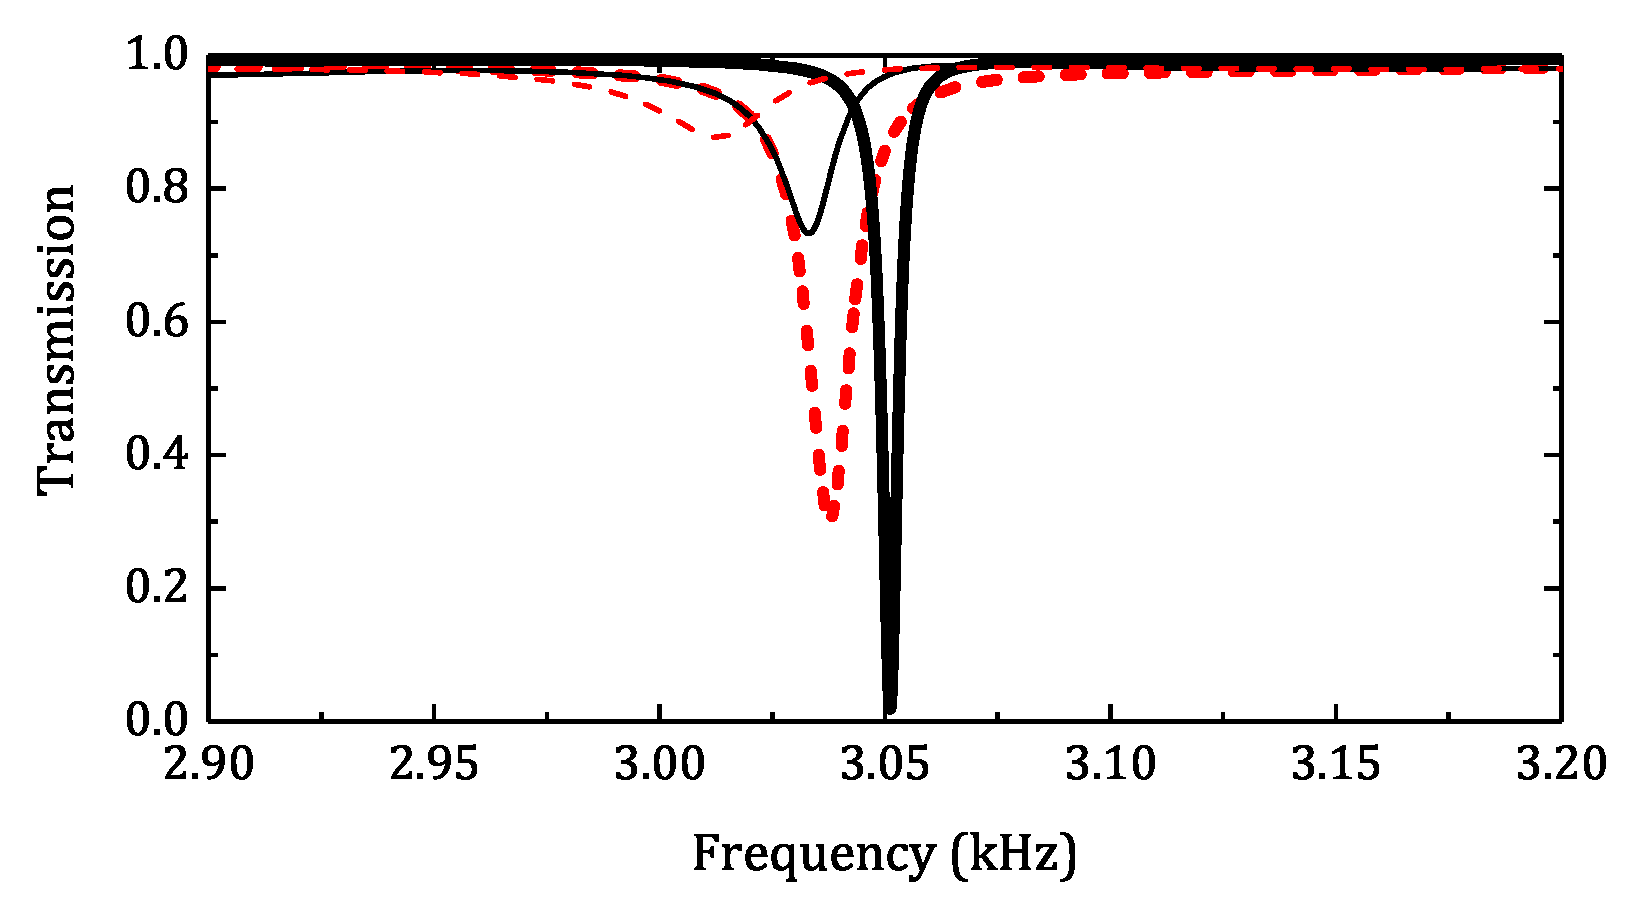
\includegraphics [width=0.9\linewidth]{tr_31_41.eps}
\caption{Transmission coefficient for the~chain of 31 (dashed red lines) and 41 (solid black lines) perforated shells. Results for inviscid and viscous air are shown by thick and thin lines respectively.}
\label{fig:tr3141Chain}
\end{center}
\end{figure}


\begin{figure}
\begin{center}
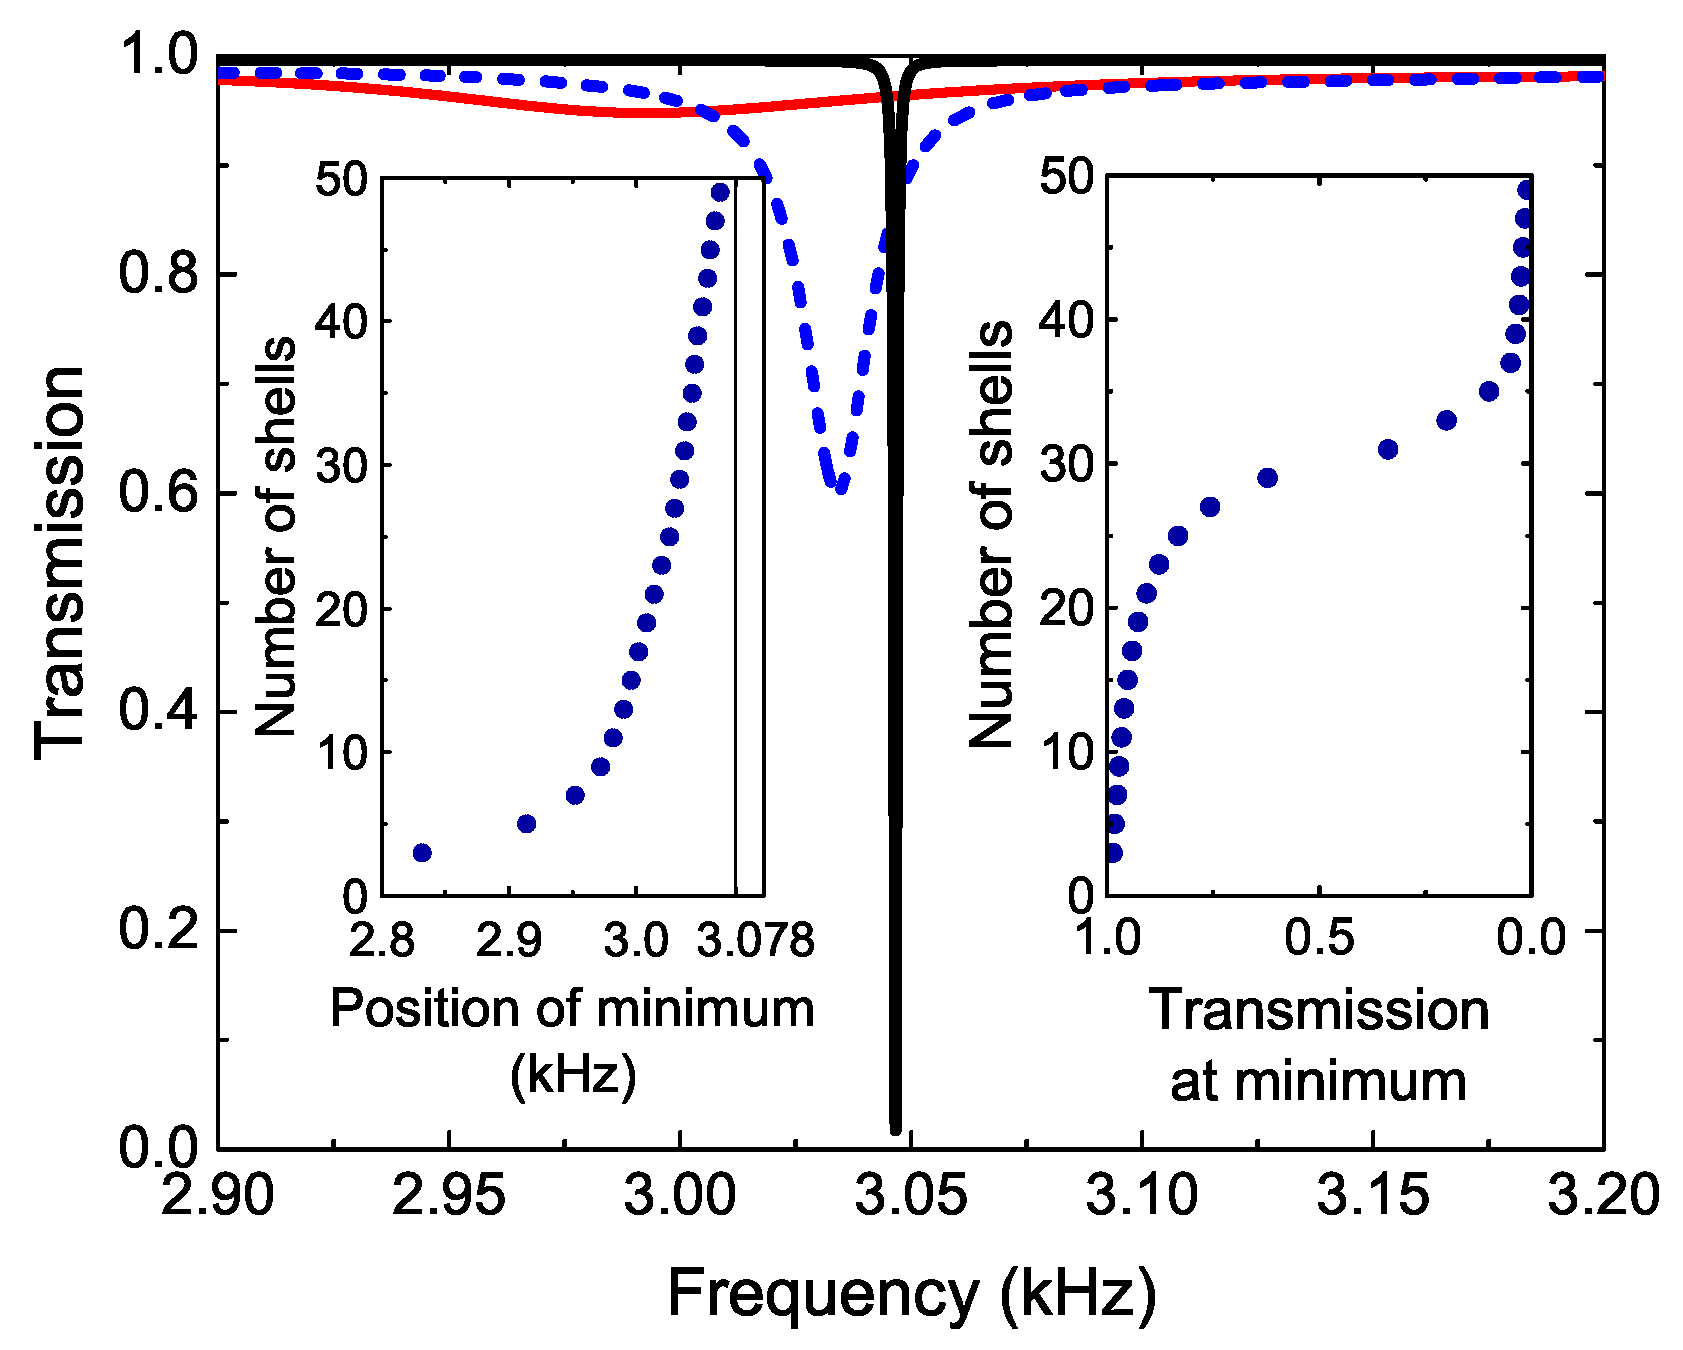
\includegraphics [width=0.7\linewidth]{tr_pos_num.eps}
\caption{Transmission coefficient for the~chain of 15 (solid red line), 29 (dashed blue line), and 37 (solid black line) perforated shells. Results are obtained for inviscid air. Inserts: position (left panel) of the~transmission minimum and its deepness (right panel) vs number of shells in the~chain.}
\label{fig:trposnumChain}
\end{center}
\end{figure}

Clearly, chains of perforated shells need to have sufficient length in order to establish the~spectrum of eigenmodes, as the~shells are weak scatterers.
Otherwise, one will not achieve any pronounced behavior of the~eigenmodes and therefore the~minima in transmission, if any, will be quite shallow.
Namely, even without the~viscosity in the~picture, there is hardly any visible minimum in the~transmission spectrum of a~15-unit chain, and it will completely disappear when the~viscosity is accounted for.
Increasing the~number of scatterers makes the~resonant minimum deeper and sharper, and also blue-shifts it.
For a~very long chain, the~minimum converges on a~specific position.
The~minima shown in \cref{fig:tr3141Chain} approach the~frequency of 3078 Hz as the~length of the~chain is increased.
This frequency, 3078 Hz, is the~first nonzero eigenfrequency at the~$\Gamma$-point in the~band structure of the~infinite periodic chain of shells in ideal air environment (see \cref{fig:dispChain}).
\cref{fig:trposnumChain} shows how the~deepness of the~resonant minimum and its position depend on the~number of units in the~chain.
It is interesting that the~position of the~resonance (left panel of \cref{fig:trposnumChain}) converges to 3078 Hz much slower than the~transmission at minimum (right panel of \cref{fig:trposnumChain}) approaches zero, making the~latter more sensitive to the~number of scatterers.


\subsection{Transmission through the~Infinite Chain}

Now, I will calculate the~transmission properties of the~infinite chain of scatterers, which requires solving the~set of equations \cref{eq:15Chain}.
In the~case of the~normal incidence of sound, the~transmission vanishes exactly at $f=3078$ Hz, which corresponds to the~frequency of the~lower level in the~doublet formed due to the~level repulsion (see \cref{fig:dispChain}(b)).
One can verify via numerical simulations that the~distribution of pressure over the~$y$-axis is symmetric (antisymmetric) for the~eigenmodes describing the~lower (higher) level of the~doublet.
It is known that an~external plane wave can only excite symmetric modes at normal incidence.
The~antisymmetric modes, in particular, the~upper level of the~doublet, cannot be excited in such geometry.
Such modes are commonly referred to as deaf modes \cite{jose,ward}.
Once the~symmetric mode in 1D chain of scatterers is directly excited, the~transmission is practically $100\%$ suppressed.
The~energy is then mostly reflected back (about 85$\%$), or equally redirected by $\pm 90^{\circ}$ towards both ends of the~chain (remaining 15$\%$).

\begin{figure}
\begin{center}
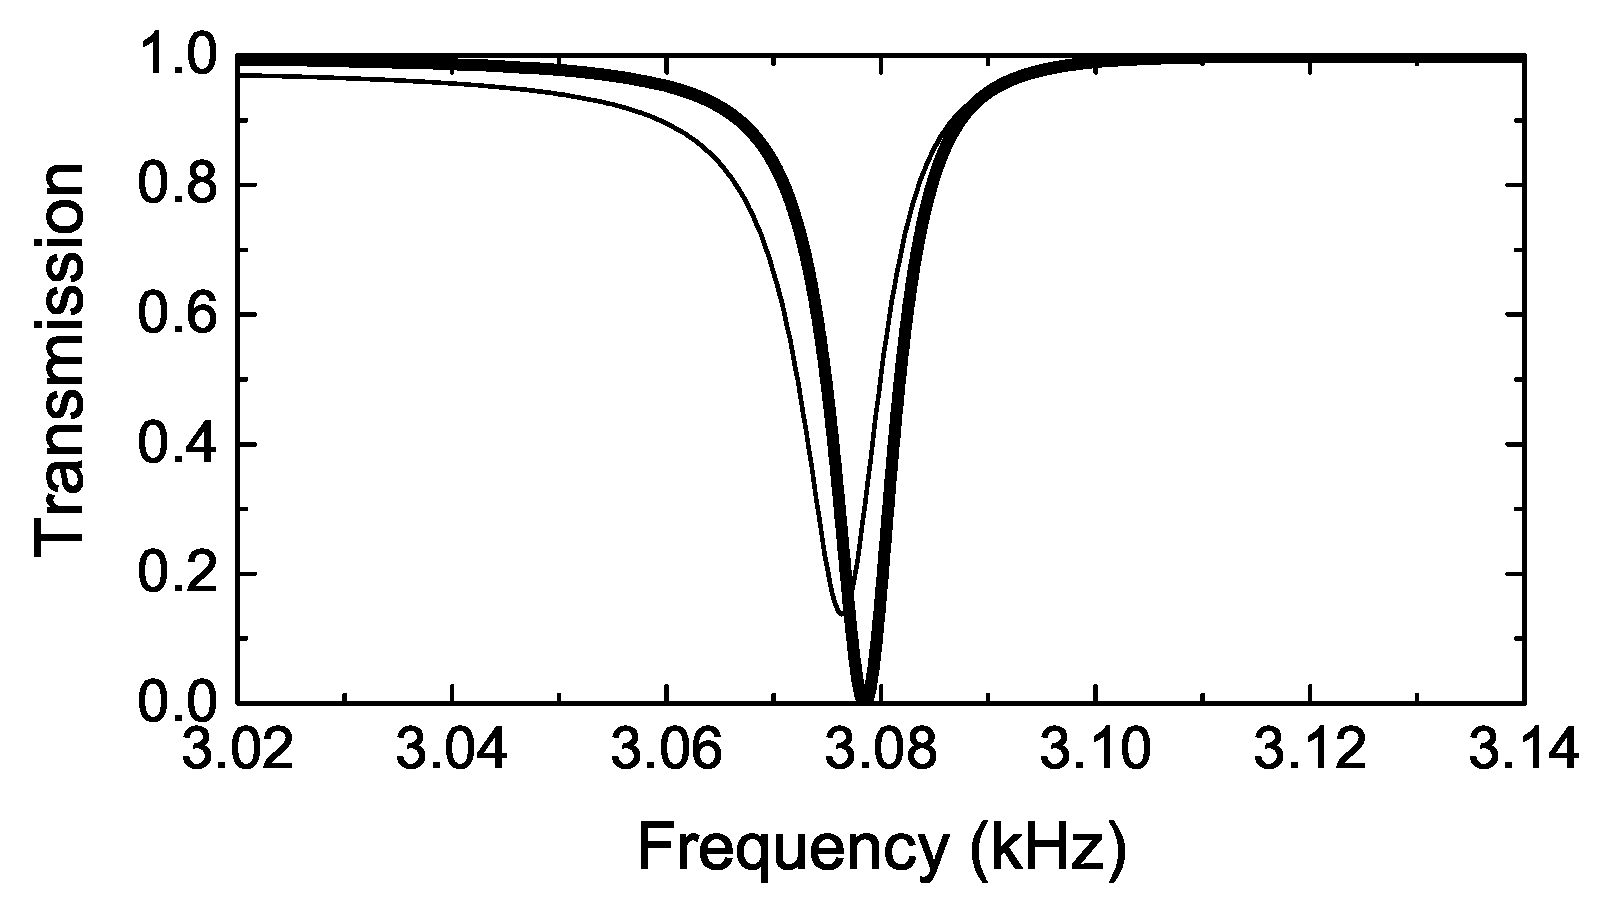
\includegraphics [width=0.7\linewidth]{tr_inf.eps}
\caption{Transmission spectrum of an~infinite chain of perforated cylindrical shells at normal incidence. Thick and thin lines are for inviscid and viscous air, respectively.}
\label{fig:trinfChain}
\end{center}
\end{figure}

Despite being a~deaf mode, an~antisymmetric mode may still be excited indirectly.
As was reported in \cite{norris1}, one may achieve the~effect of redirection of sound in a~sonic crystal of elastic rods due to the~Poisson-like effect.
Namely, the~incoming sound excited the~flexural modes of the~rods, and those modes coupled to the~antisymmetric deaf modes via evanescent modes. Such indirect excitation allowed only a~maximum of $46\%$ of acoustic energy to be reflected or redirected at the~frequency of the~mid-gap.

It is important to note from \cref{fig:trinfChain} that the~resonance in a~chain surrounded by viscous air is not significantly altered by dissipation, specifically, there is only a~slight red shift and almost no broadening of the~resonance (the~width remains approximately $\Delta f=30$ Hz).
As is seen from \cref{fig:tr3141Chain} and \cref{fig:trposnumChain}, the~most important factor defining the~shape of the~resonant minimum is the~length of the~chain.
The~viscosity is then does not qualitatively change the~observed phenomena, and only weakly contributes to the~quantitative results.
Due to viscosity, the~transmission at the~resonance does not reach zero and becomes finite.
Still, about $80\%$ of acoustic energy experiences either reflection or redirection as the~symmetric leaky modes of the~chain are excited.
%%
The~leaky modes are not proper spectral modes, and one benefits from this fact since such modes can be directly excited by external sound due to their interaction with the~environment.
Moreover, the~inequality $\im f \ll \Delta f \ll \re f$ holds, and for that reason the~resonant excitation is well established.


When the~external acoustic plane wave is incident at an~angle, there is no symmetry of the~incoming wave over the~$y$-axis, which makes the~excitation of both symmetric and antisymmetric eigenmodes possible.
For that reason, the~two minima appear in the~transmission spectra in \cref{fig:trangleChain}.
In order to find the~position of each minimum, the~wave vectors of the~incoming sound $\mathbf{k}$ and the~eigenmode $q$ must satisfy the~following relation:
\begin{equation}
\label{eq:18Chain}
k_{y}=(2\pi f/c_0) \sin \theta = q(f).
\end{equation}
The~latter condition, which requires matching of the~tangential components of the~wave vectors, is the~mathematical form of the~phenomenon known as the~Wood's anomaly \cite{maystre}.
As an~example, the~resonant minimum in the~transmission spectrum \cref{fig:trinfChain} can be considered as a~Wood's anomaly since at the~resonant frequency 3078 Hz, the~wavelength of sound in air is 11.1 cm, which closely matches the~period of the~chain $d=11$ cm \cite{garcia1}.
In the~reduced zone scheme, the~condition \cref{eq:18Chain} can be satisfied for multiple frequencies, depending on the~angle of incidence $\theta$.
For normal incidence, $\theta=0^{\circ}$, the~corresponding value of the~wave vector is $q=0$, which formally enables any dispersion band to be excited by external sound.
Together with the~symmetry consideration one concludes that normal incidence only triggers excitation of lower levels of the~doublets at the~$\Gamma$-point.

In general, \cref{fig:dispChain} shows the~points of crossing of the~straight dashed lines given by $q=2\pi f \sin\theta/c_0$ with the~dispersion bands, where the~condition \cref{eq:18Chain} is satisfied.
The~three dashed lines correspond to the~angles of incidence $\theta = 5^{\circ}$, $\theta = 10^{\circ}$ and $\theta = 15^{\circ}$.
For $\theta = 5^{\circ}$, the~first two crossings occur at $f \approx 2.85$ kHz and $f \approx 3.40$ kHz.
Consequently, the~transmission minima in \cref{fig:trangleChain} are observed near these frequencies.
These two minima are separated by the~interval of about 550 Hz, which is significantly larger than either the~width of each minimum or the~width of the~doublet at the~$\Gamma$-point.
The~latter fact makes each minimum well-resolved, and is explained by the~difference in the~dispersion of the~two bands.
Since the~upper (antisymmetric) and the~lower (symmetric) bands are the~continuations of the~doublet levels at the~$\Gamma$-point, they exhibit normal and anomalous dispersion, respectively, meaning the~separation between their respective eigenfrequencies is increased away from the~$\Gamma$-point.


\begin{figure}
\begin{center}
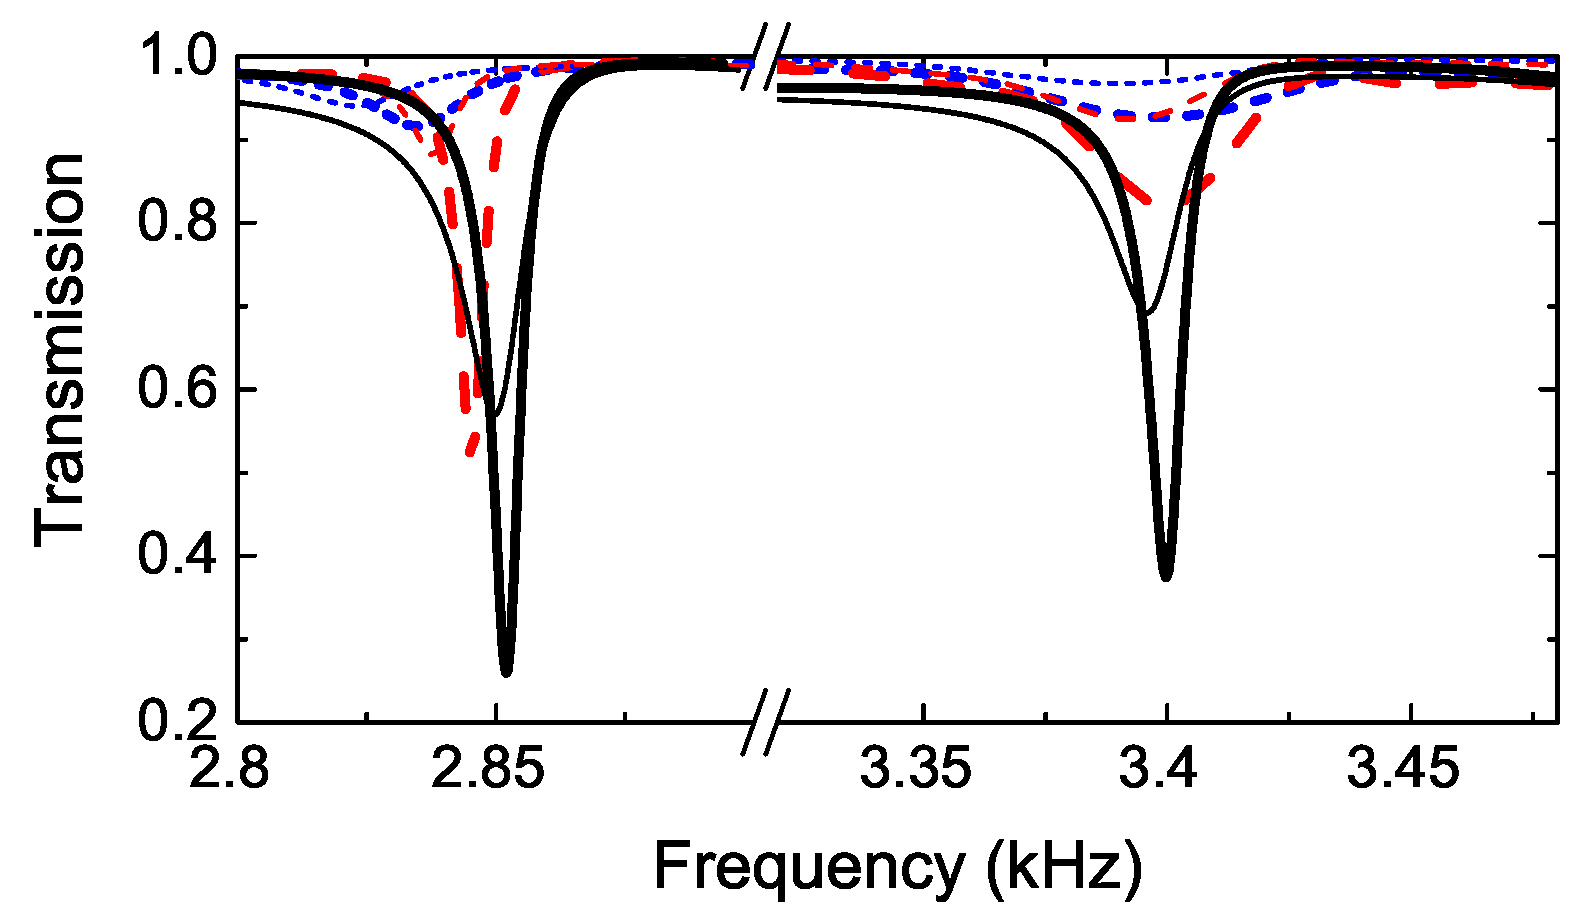
\includegraphics [width=0.7\linewidth]{tr_angle5.eps}
\caption{Transmission spectrum at oblique incidence, $\theta = 5^{\circ}$. Blue short-dashed, red long-dashed, and black solid lines are for the~chains containing 61, 121, and infinite number of cylindrical shells, respectively. Thick and thin lines show the~results for inviscid and viscous air. Note that two resonances are separated by $\approx 550$ Hz in frequency (compare to the~doublet width $35$ Hz).}
\label{fig:trangleChain}
\end{center}
\end{figure}


An~interesting anomaly arises in the~scattering of sound by the~chain of perforated shells as a~result of the~bands having different dispersion.
One can see that the~direction of the~phase velocities for both eigenmodes is the~same as the~direction of the~wave vector ${\bf q} = q\hat{y}$.
The~group velocity, however, acquires its sign from the~slope of the~corresponding band curve, so for the~lower band it is opposite to $\bf q$.
As the~group velocity points in the~direction of the~energy flow, it appears that the~scattering of the~incoming wave occurs in the~"wrong" direction.

\cref{fig:polarUChain} and \cref{fig:polarDChain} visualize the~angular distribution of intensity of scattered sound for the~angle of incidence $\theta = 5^{\circ}$.
In \cref{fig:polarUChain}, the~frequency of 3.40 kHz is selected for the~incoming wave to allow coupling with the~upper dispersion band (see \cref{fig:dispChain}).
The~scattered sound propagates almost exclusively in the~direction of the~parallel component $k_{y}\hat{y}$ of the~wave vector in the~incoming wave, due to the~normal dispersion of the~band.
In contrast with that, the~scattering at the~frequency of $f=2.85$ kHz, where the~matching condition \cref{eq:18Chain} holds for the~lower band with anomalous dispersion, occurs in the~direction against $k_{y}\hat{y}$ and produces anomalous pattern for the~scattered field (see \cref{fig:polarDChain}).

Both \cref{fig:polarUChain} and \cref{fig:polarDChain} also show the~results obtained for viscous air by green dashed lines.
Due to viscosity of air, the~scattered sound is of lower intensity in all the~directions.
Despite that, the~coupling to the~eigenmodes remains effective, and the~spikes of intensity in the~normal and "wrong" directions remain well-pronounced.


\begin{figure}
\begin{center}
\includegraphics [width=0.9\linewidth]{polar_3400.eps}
\caption{Polar diagram showing distribution of intensity of scattered sound of frequency $f = 3400$ Hz (upper band in the~doublet having normal dispersion). Solid-red and green-dashed lines are for inviscid and viscous air, respectively. Black arrow shows the~direction of the~incident wave. An~essential part of scattered sound wave propagates along the~chain in the~direction of the~wave vector $\bf k_{\|}$. Note logarithmic scale along radius.}
\label{fig:polarUChain}
\end{center}
\end{figure}



\begin{figure}
\begin{center}
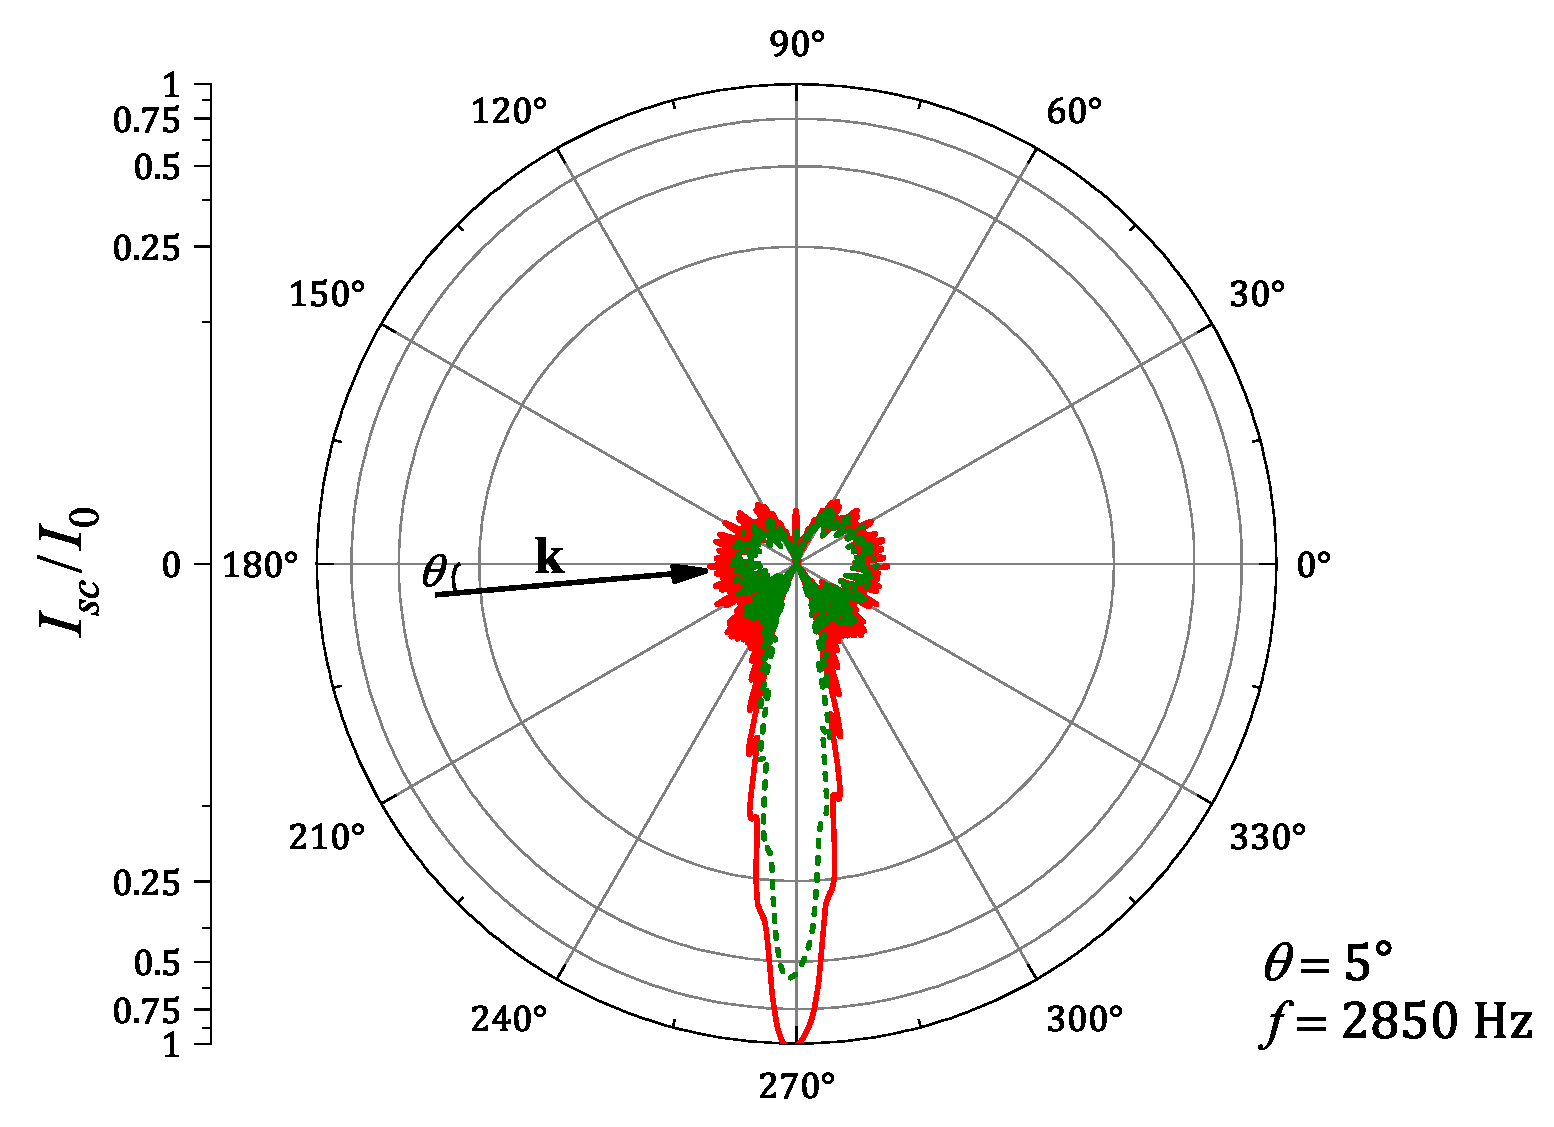
\includegraphics [width=0.9\linewidth]{polar_2850.eps}
\caption{The~same as in \cref{fig:polarUChain} but for the~frequency $f=2850$ Hz, corresponding to the~lower band of the~doublet, having anomalous dispersion. In this case the~scattering occurs in the~"wrong" direction, i.e., opposite to $\bf k_{\|}$.}
\label{fig:polarDChain}
\end{center}
\end{figure}


\begin{figure}
\begin{center}
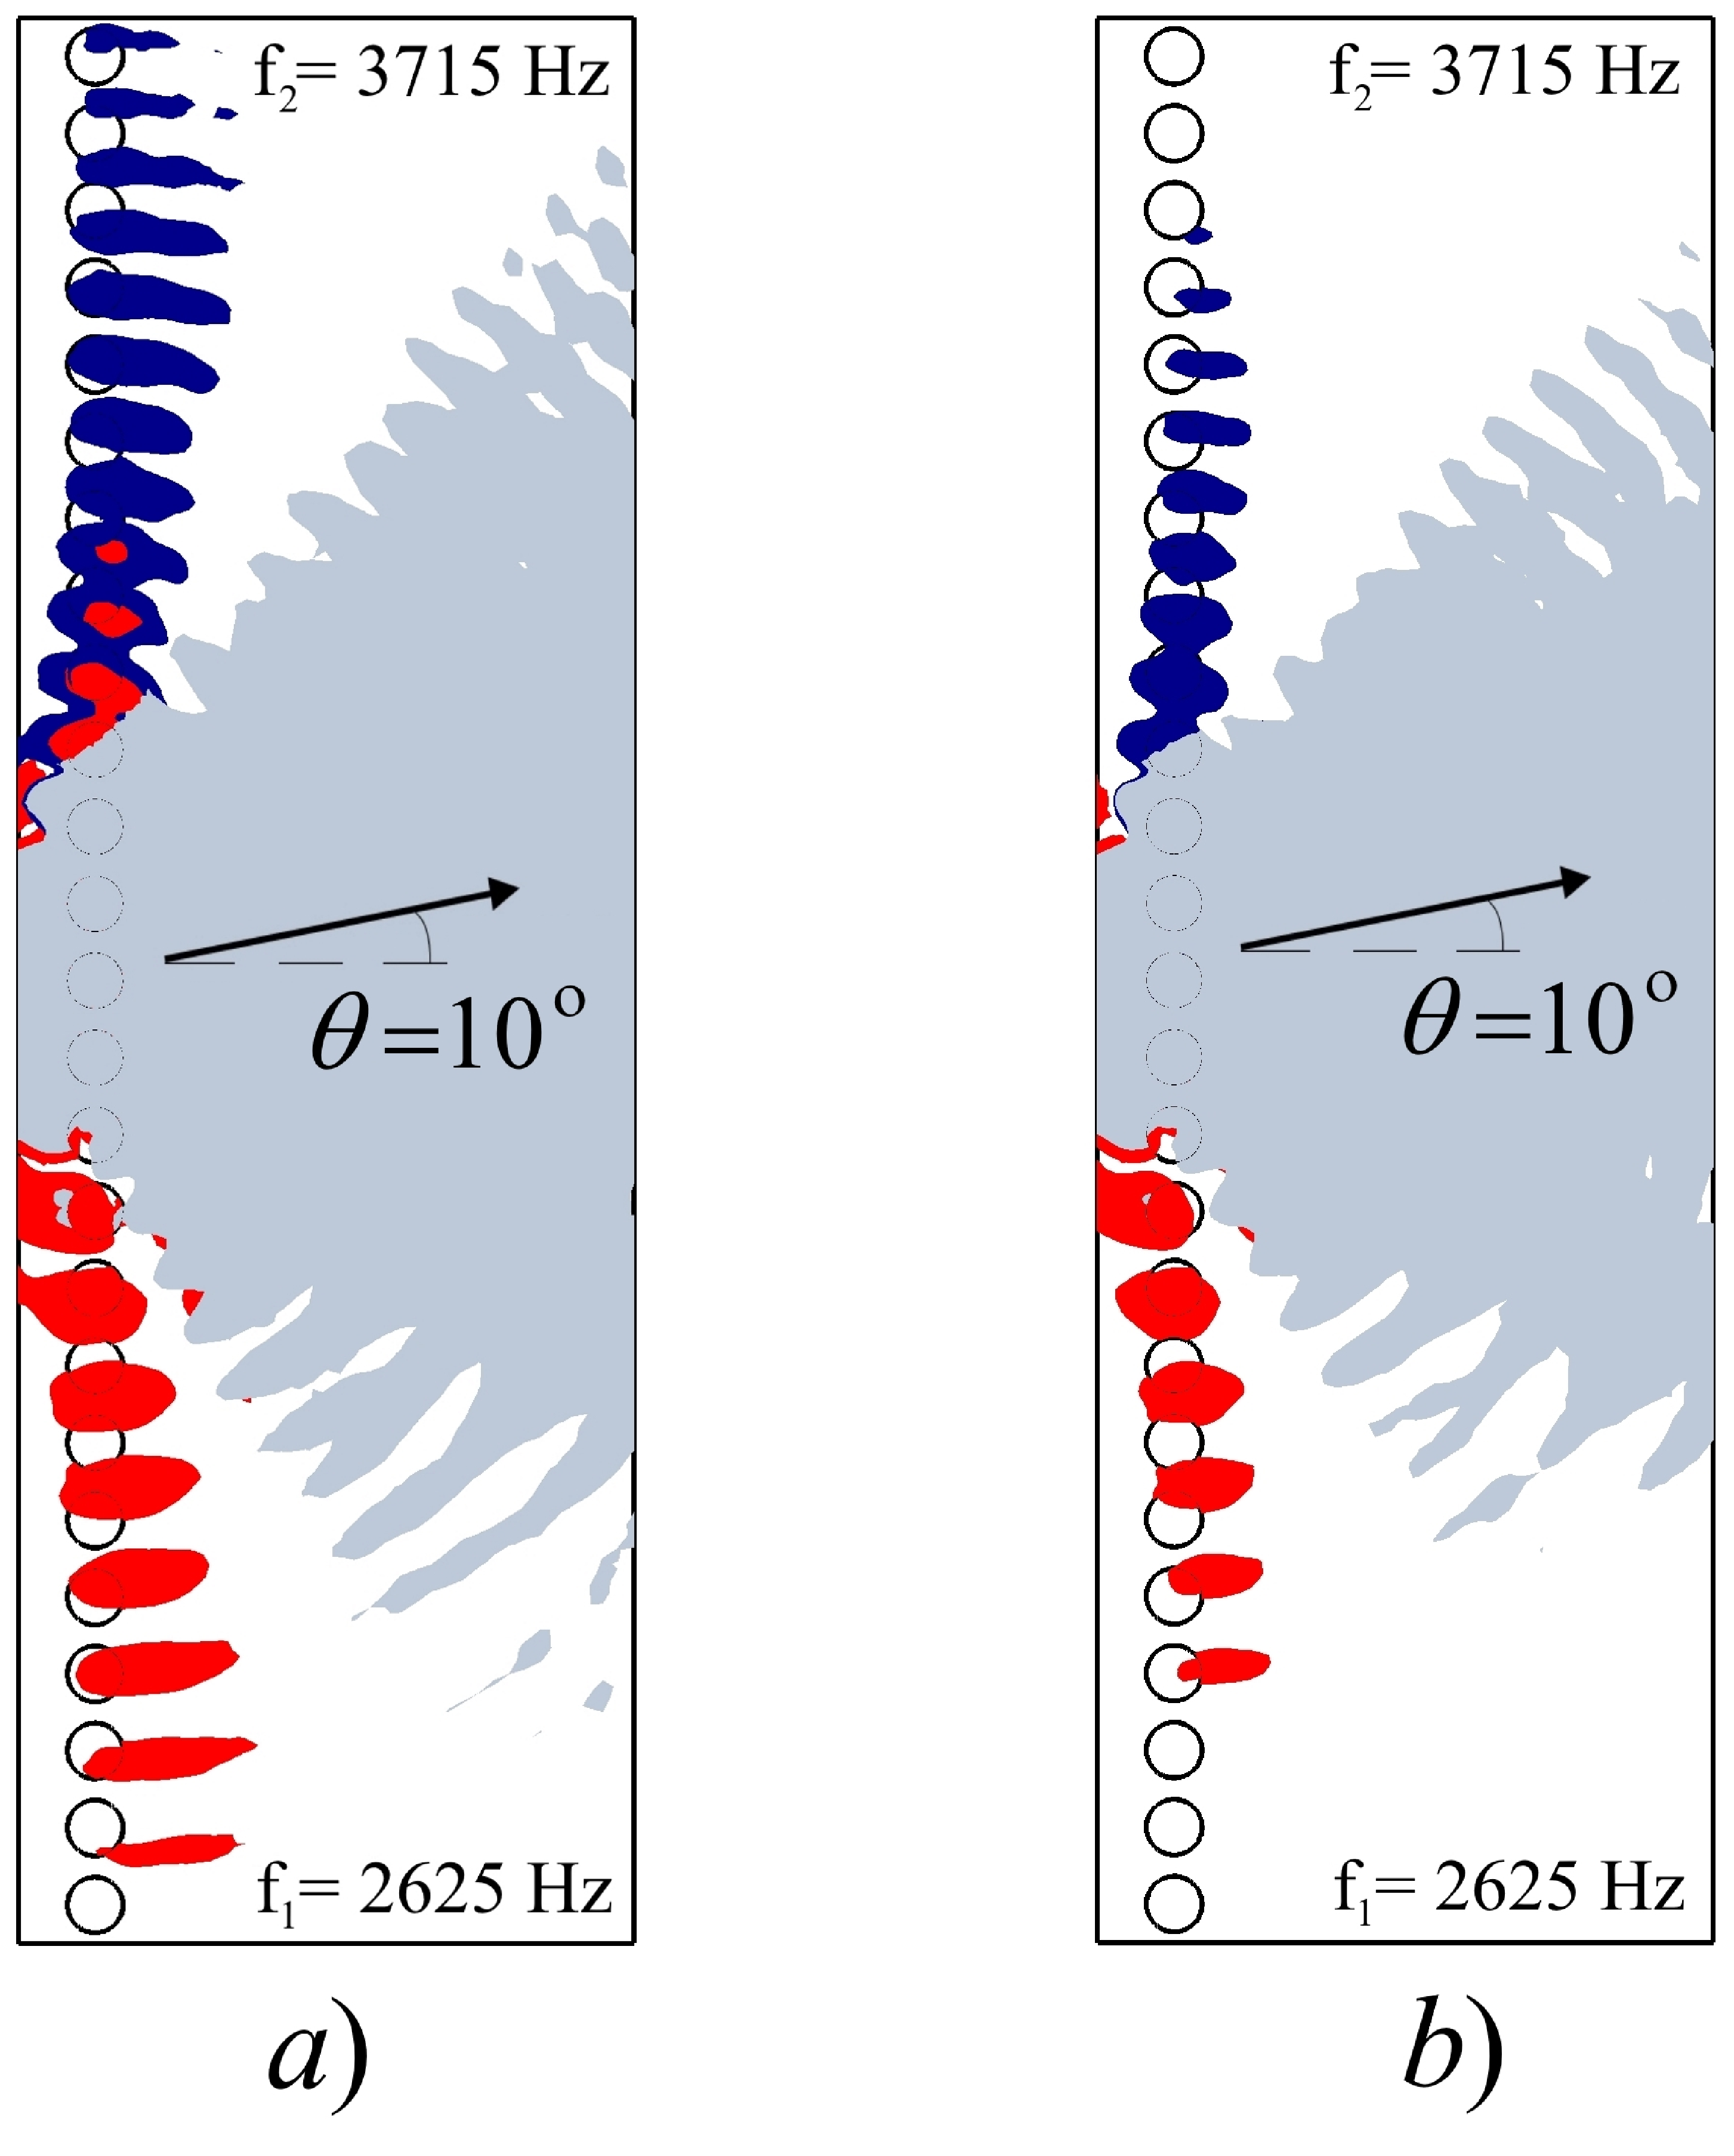
\includegraphics [width=0.7\linewidth]{bifreq_split.eps}
\caption{Distribution of intensity of a~bi-frequency signal (with $f_1=2625$ Hz and $f_2=3715$ Hz) transmitted through a~chain of 25 perforated shells. The~angle of incidence is $10^{\circ}$ and the~background air is inviscid (a) and viscous (b). The~central part of the~diffraction pattern (shown in grey) is a~mixture of two sound waves with frequencies $f_1$ and $f_2$.  The~red and blue fringes are the~split monochromatic components. The~low-frequency component (red) exhibits anomalous scattering, propagating against the~"natural" direction. The~high-frequency component (blue) follows the~"natural" direction due to its normal dispersion.}
\label{fig:bifreqChain}
\end{center}
\end{figure}


There is no great difference between the~intensities of the~normal and anomalous scattering for the~angles of incidence $\theta \geq 5^{\circ}$.
The~results in \cref{fig:trinfChain} serve as the~evidence for the~latter claim, showing that the~values of the~transmission coefficients in the~minima differ by $10\%$, with the~lower-frequency minimum being deeper.
For smaller angles $\theta$, however, the~eigenmode with normal dispersion produces much weaker minimum as it becomes a~deaf mode towards $\theta = 0^{\circ}$, and as a~result the~anomalous scattering dominates.
When $\theta \rightarrow 0^{\circ}$, the~frequency interval between two resonant minima in the~transmission spectra approaches the~width of the~doublet, which may be hard to see from the~plots as the~minimum corresponding to normal scattering vanishes completely.

The~plots in \cref{fig:trinfChain}-\cref{fig:polarDChain} clearly demonstrate the~effect of redirection of incoming sound by an~angle of about $90^{\circ}$.
This becomes possible in a~chain of weak scatterers when the~frequency and the~angle of incidence satisfy the~matching condition \cref{eq:18Chain}.


\subsection{Splitting of Acoustic Signal}

Additionally, the~chain of perforated shells may serve as a~splitter of a~bi-frequency acoustic signal.
Let us consider an~acoustic beam which is created by mixing two monochromatic sound waves and is incident on the~chain at a~certain angle $\theta$.
The~described beam will produce two monochromatic signals propagating along the~chain in the~opposite directions, provided that both frequencies of its components are solutions of \cref{eq:18Chain}.
In the~case of almost normal incidence, the~detuning between the~components needs to be much smaller than their frequencies (such bi-frequency signal is called a~beat).
Due to closeness to the~$\Gamma$-point, the~redirection of the~high-frequency component is suppressed and the~overall efficiency of splitting is reduced.

In \cref{fig:bifreqChain}, a~bi-frequency signal is incident at an~angle of $10^{\circ}$ on the~finite-length chain containing 25 perforated shells.
The~two monochromatic components of the~signal have frequencies of $2625$ Hz and $3715$ Hz, respectively, which are the~frequencies of the~two eigenmodes of the~chain that can be excited by the~wave incident at $10^{\circ}$ (see \cref{fig:dispChain}).
A~substantial part of acoustic energy propagates through the~chain, as the~angle of incidence is not very small and the~number of shells is not very large.
Nevertheless, one can observe a~clear pattern of split fringes towards either end of the~chain, for both ideal (\cref{fig:bifreqChain}a) and viscous (\cref{fig:bifreqChain}b) air.

The~chain of perforated shells, being a~purely mechanical system, demonstrates quite good efficiency of splitting.
The~amounts of energy that are converted into the~low-frequency component, propagating down (anomalous scattering), and high-frequency component, propagating up (normal scattering), are as high as $8\%$ ($5\%$) and $10\%$ ($7\%$), respectively, for the~chain in ideal (viscous) air environment.
%In \cref{fig:bifreqChain} we show the~splitting of a~bi-frequency signal when it hits the~chain at the~angle of $10^{\circ}$ in ideal (panel (a)) and viscous (panel (b)) air. The~frequencies of the~monochromatic components, $2625$ Hz and $3715$ Hz, are obtained from the~band diagram in \cref{fig:dispChain}. Since the~chain contains only 25 shells and the~angle of incidence is not very small, the~essential part of acoustic energy propagates directly through the~chain. Nevertheless, a~clear pattern of split fringes is observed even for viscous air.
%The~efficiency of splitting is quite good for a~pure mechanical splitter, for ideal (viscous) air $8\%$ ($5\%$) of energy is converted into the~low-frequency component, propagating down (anomalous scattering) and $10\%$ ($7\%$) of energy is converted into the~higher-frequency component, propagating up (normal scattering).



%++++++++++++++++++++
\section{Summary}

This chapter presents a~rigorous study of the~interaction between the~acoustic waves and the~periodic chain of thin perforated cylindrical shells, which results in redirection and splitting of incident sound.
The~problem of diffraction of sound by the~periodic arrangement of shells is solved analytically in impedance approximation, applicable for situations with both ideal and viscous background fluid.
The~transmission coefficient is calculated for infinite and finite-length chains within a~wide range of frequencies, and agrees well with earlier numerical and experimental results reported in \cite{garcia1} and further expanded in \cite{victorthesis}.

To gain more insights into the~predicted phenomena, the~dispersion equation for the~infinite periodic chain is derived, and the~eigenmodes are then numerically obtained for aluminum scatterers in air.
Weak coupling between the~scatterers and sound causes the~eigenmodes to be leaky modes, propagating with phase velocity close to the~speed of sound in air and slowly radiating energy away from the~chain.
The~eigenmodes can be resonantly excited by the~incident sound, leading to sharp minima in the~transmission spectrum at the~frequencies satisfying specific matching condition.

At normal incidence, the~coupling of a~monochromatic acoustic wave is only possible to the~symmetric chain eigenmode, which results in a~single deep minimum in the~transmission.
The~antisymmetric mode, no matter how close to the~symmetric mode frequency-wise, cannot be excited via normal incidence.
With this, equal parts of the~incoming sound are redirected in both directions along the~chain.

When the~incidence is oblique, the~external wave can couple to both symmetric and antisymmetric modes, and that causes two deep minima to appear in the~transmission spectrum.
These minima are well-resolved even for viscous air.
Since the~symmetric and antisymmetric modes exhibit anomalous and normal dispersion, respectively, the~anomalous scattering is strongly manifested in the~system.
The~scattering of acoustic energy along the~chain in the~opposite direction with respect to the~direction of incidence is shown to be a~strong effect, caused by the~resonant coupling between the~external sound and the~symmetric mode.
Consequently, the~chain of perforated scatterers can effectively serve as a~sound splitter.
Namely, a~sound beam consisting of two (or more) monochromatic components, which match the~frequencies of symmetric and antisymmetric modes and thus have different dispersion, is split into two parts propagating in opposite directions along the~chain.

In order to back the~theoretical predictions, one needs to perform further experimental work focused on designing and testing devices for filtering and splitting of sound waves at selected frequencies.


%In summary, we have demonstrated redirection and splitting of sound waves impinging a~periodic chain of thin perforated cylindrical shells.
%These conclusions have been obtained using an~analytical approach to the~problem of diffraction of sound by a~periodic chain of perforated cylindrical shells, which has been developed here.
%Scattering at the~shells is described in impedance approximation, which is applicable for both lossless and viscous background fluid.
%The~dispersion equation for the~eigenmodes of an~infinite periodic chain is derived and its complex solutions are obtained numerically for aluminum perforated shells in air.
%Since these shells are only weak scatterers of sound, the~eigenmodes are leaky waves propagating with phase velocity close to the~speed of sound in air, and they slowly decay due to dissipation and radiation.
%The~transmission coefficient is calculated for infinite and finite-length chains within a~wide range of frequencies.
%At normal incidence, the~coupling to the~lowest symmetric eigenmode gives rise to a~deep minimum in the~transmission.
%In this geometry, the~antisymmetric mode, which is close in frequency, is not excited and the~incoming wave is equally redirected along the~chain in both directions.
%At oblique incidence, the~external wave can be coupled to both symmetric and antisymmetric modes that leads to two deep minima in the~transmission spectrum which are well-resolved for viscous air.
%Here anomalous scattering is strongly manifested because the~symmetric mode exhibits anomalous dispersion while for the~antisymmetric one the~dispersion is normal.
%We find that resonant coupling of external sound to the~symmetric mode results in strong scattering  of acoustic energy along the~chain in the~"wrong" direction with respect to the~direction of incidence. Finally, we show that due to different dispersion of symmetric and antisymmetric modes a~sound beam consisting of two (or more) monochromatic components can be effectively split into two parts propagating in opposite directions along the~chain.
%Each part is a~monochromatic wave with the~frequency resonating with either symmetric or antisymmetric eigenmode.
%Further experimental work should be performed in order to support our theoretical predictions, which foresee useful devices for the~filtering and splitting of sound waves at selected frequencies.




%%% Local Variables: 
%%% mode: latex
%%% TeX-master: "dissertation"
%%% End: 
